\documentclass[14pt]{article} % класс документа
%Преамбула документа
\usepackage[T2A]{fontenc} 
% задаём кодировку шрифтов
\usepackage[utf8]{inputenc} 
% задаём кодировку файла% задаём правила переносов для русского языка
\usepackage[english,russian]{babel}
% Текст документа
\usepackage{amsmath}
\usepackage{amsfonts}
\usepackage{amssymb}
\usepackage[colorlinks, urlcolor=blue]{hyperref}
\usepackage{graphics, graphicx}
\usepackage{enumerate}
\usepackage[14pt]{extsizes}
\usepackage{multicol}
\usepackage{subcaption}


\usepackage{amssymb,amsmath}
\textheight=24cm
\textwidth=16cm
\oddsidemargin=0pt 
\topmargin=-1.5cm
\parindent=24pt
\parskip=0pt
\tolerance=2000 
\flushbottom
%\def\baselinestreth{1.5}

\begin{document}
\begin{titlepage}
	\thispagestyle{empty}
	\begin{center}
		Московский~государственный~университет~имени~М.\,В.\,Ломоносова\\
		Факультет вычислительной математики и кибернетики\\
		Кафедра математических методов прогнозирования\\
	\vfill

	\textbf{\Large Отчет по градиентным методам \\ обучения 
	линейных моделей}\\[4cm]
	\end{center}
	\hfill
	\begin{minipage}{0.3\textwidth}
		\large
		\raggedleft
		\textbf{Выполнил:\\[2mm]}
		\raggedleft
		Cтудент 3 курса\\
		Н.\,А.\,Панин
	\end{minipage}
	\vfill
	\begin{center}
		\large \bf Москва\\2022
	\end{center}

\end{titlepage}
\newpage
\section{\huge Введение}
В задачах машинного обучения часто возникает необходимость минимизировать 
гладкие выпуклые функционалы. Задача нахождения минимума у таких функционалов
хорошо решается градиентными методами.

В данной работе рассматривалась
логистическая регрессия ({\itshape Logistic regression})~- линейный классификатор, 
главным преимуществом которого является корректное определение вероятности 
принадлежности объекта определенному классу. В логистической регресии необходимо 
минимизировать эмпирический риск с логистической функцией потерь.
На примере этого функционала была решена задача минимизации эмпирического 
риска для данных, содержащих в качестве признака комментарии из википедии, 
а в качестве целевой  переменной метку "токсичный"$\backslash$"не токсичный". Рассматривались 
такие градиентные методы как: {\itshape градиентный спуск} \ и {\itshape стохастический градиентный спуск}.
Исследовались оптимальные параметры данных методов для минимизации функции потерь. 
Оценивалось влияние предобработки текста с помощью лемматизации и выкидывания 
стоп-слов на точность предсказания, время работы, размер признакового пространства. 
Также были рассмотрены два метода векторизации: BagOfWords и Tf-Idf. В конце были 
проанализированы и указаны общие черты объектов, на которых была допущена ошибка.
\newpage
\section{\huge Теоретическая часть}
Рассмотрим задачу бинарной логистической регрессии. Пусть дана обучающая выборка
$X=(x_i, y_i)_{i=1}^N$, где $x_i \in \mathbb{R}^D$, $ y_i \in \mathbb{Y}=\{ 1, -1\}$, 
$\omega \in \mathbb{R}^D$~-- вектор весов.
\begin{enumerate}
	\item Функция потерь будет иметь следующий вид:
		\[
			Q(X, y, \omega)=\frac{1}{N}\sum_{i=1}^N\ln\bigl(1+\exp(-y_i\langle x_i, \omega\rangle)\bigr)\to \min_{\omega}
		\]
		Найдем дифференциал функции потерь по $\omega$:
		\[
			d_wQ(X, y, \omega)=-\frac{1}{N}\sum_{i=1}^N\frac{\exp(-y_i\langle x_i, \omega\rangle)y_ix_i^Td\omega}
			{1 + \exp(-y_i\langle x_i, \omega\rangle)}
		\]
		$$
			\Longrightarrow \bigtriangledown_wQ(X, y, \omega)=\Bigl\{ \sigma(z) = \frac{1}{ 1+ e^{-z} }\Bigr\}=
			-\frac{1}{N}\sum_{i=1}^Nx_iy_i\sigma(-y_i\langle x_i, w\rangle),
		$$
		где $\sigma(z)$ - сигмоида
	\item Рассмотрим задачу мультиноминальной логистической регрессии, т.е. 
	$\mathbb{Y}=\{1,2,\dots,K\}$. Тогда функция потерь будет иметь следующий вид:
	$$
		Q(X, y, \omega)=-\frac{1}{N}\sum_{i=1}^N\ln\Bigl(\frac{\exp(\langle x_i, 
		\omega_{y_i}\rangle)}{\sum_{k=1}^K\exp(\langle x_i, \omega_k\rangle)}\Bigr)
		=
	$$
	$$
		=\frac{1}{N} \sum_{i=1}^N\Biggl[\ln\Bigl(\sum_{k=1}^K\exp(\langle x_i, \omega_k\rangle)\Bigr)
		- \langle x_i, \omega_{y_i}\rangle\Biggr] \to \min_{\omega_1,\omega2,\dots,\omega_K 
		\in \mathbb{R}^{D}}
	$$
	Градиентом в данном случае будет матрица размера $D \times K$:
	$$
		dQ_{w_j}(X, y, \omega) = \frac{1}{N}\sum_{i=1}^N\Biggl[
			\frac{\sum_{k=1}^K\exp(\langle x_i, \omega_k\rangle)d\langle 
				x_i, \omega_k\rangle}{\sum_{k=1}^K\exp(\langle x_i, \omega_k\rangle)} -
				d\langle x_i,\omega_{y_i}\rangle\Biggr] =
	$$
	$$
		= \frac{1}{N}\sum_{i=1}^N\Biggl[
			\frac{\exp(\langle x_i, \omega_j\rangle)
				x_i^Td\omega_j}{\sum_{k=1}^K\exp(\langle x_i, \omega_k\rangle)} -
				x_i^T[y_i=j]dw_j\Biggr]
	$$
	$$
	\Longrightarrow \bigtriangledown_{w_j}Q(X, y, \omega) = 
		\frac{1}{N}\sum_{i=1}^N\Biggl[
			\frac{\exp(\langle x_i, \omega_j\rangle)
				x_i}{\sum_{k=1}^K\exp(\langle x_i, \omega_k\rangle)} -
				x_i[y_i=j]\Biggr]
	$$
	$\bigtriangledown_{w_j}Q(X, y, \omega)$ - это $j$-й столбец этой матрицы.

	\item Покажем связь между бинарной логистической регрессией и мультиноминальной
	 логистической регресии, а именно докажем, что бинарная логистическая регрессия 
	 является частным случаем мультиноминальной.
	 Действительно, для бинарной логистической регрессии:
	$$
	 	\mathbb{P}(y=1|x) = \sigma(\langle w, x\rangle)
	$$
	Для мальтиноминальной логистической регрессии при $K=2$:
	$$
	 	\mathbb{P}(y=1|x) = \frac{\exp(\langle\omega_1, x\rangle)}
		{\exp(\langle\omega_1, x\rangle) + \exp(\langle\omega_{-1}, x\rangle)}=
		\frac{1}{1 +  \exp(\langle\omega_{-1} - \omega_{1}, x\rangle)}=
	$$ 
	$$
		= \sigma(\langle\omega_{1} - \omega_{-1}, x\rangle)
	$$
	Так как задача нахождения оптимального решения в случае бинарной 
	и мультиноминальной логистической регрессии сводится к максимизации 
	функции правдоподобия, а вероятности равны, если положить $\omega = \omega_1
	- \omega_{-1}$, то отсюда следует эквивалентность данных методов при $K=2$.

	
\end{enumerate}
\section{\huge Список экспериментов}
Перед проведением экспериментов была проведена предобработка текстов: приводились слова к нижнему регистру, не буквы и не цифры удалялись и заменялись на пробелы.

Обучающая выборка была перемешена и разделена на валидационную и обучающую в отношении 1 : 4.

 Значения некоторых параметров не изменялись почти во всех экспериментах. Если эти значения будут меняться, то это будет отдельно оговорено. Перечислим значения этих параметров по умолчанию:
\begin{itemize}
	\item 
	Максимальное количество итераций(эпох в случае стохастического градиентного спуска)[{\sl max\_iters}]\footnote{Далее для сокращения записи в случае {\itshape градиентного спуска} будем писать {\bfseries GD}, а в случае {\itshape стохастического градиентного спуска} {\bfseries SGD}}: 100
	\item  
	Точность[{\sl tolerance}]: $10^{-10}$
	\item
	Коэффициент $l_2$-регуляризации: 0.1
	\item Размер батча(подвыборки для подсчета градиента в SGD)[{\sl batch\_size}]:~10000 
	\item Частота обновлений "истории"(время, accuracy и значение функции потерь) SGD: 1 эпоха
\end{itemize}

Рассмотрим формулу итерационного нахождения минимума:
\begin{equation}
	\omega_{k+1} = \omega_k - \frac{1}{L}\eta_k\sum_{i=1}^L\bigtriangledown_\omega Q(X,y,\omega_k),
\label{grad}
\end{equation}
где $L$ - это либо {\sl batch\_size}, либо размер выборки $X$.

В качестве темпа обучения({\itshape learning rate}) бралась 
\begin{equation}
	\eta_k =\frac{\alpha}{k^\beta}\label{step}
\end{equation}
\subsection{Эксперимент 0. Анализ  аналитической и разностной формулы градиента  для логистической регрессии.}
\subsubsection{Дизайн эксперимента}
В ходе данного эксперимента производилась разностная проверка градиента, а именно, использовалось следующее:
	$$
		[\nabla f(x)]_i \approx \frac{f(x + \varepsilon e_i) - f(x)}{\varepsilon},
	$$
	где $e_i = (0,\dots,0,1,0,\dots,0)$; $i$ --  индекс, в котором стоит единица, а
	$\varepsilon \sim \sqrt{\varepsilon_{mach}}$, где $\varepsilon_{mach}$ - машинная точность ($\approx\!10^{-16}$). Причем в нашей задаче в качестве
	$f(\omega)$ будет $Q(X, y, \omega)$. В качестве параметров($X$, $y$) и переменной($w$) брались следующие значения:
	\begin{itemize}
		\item $X \sim \mathcal{U}(-100, 100)$, $X \in \mathbb{R}^{m \times n}$, где $m$ и $n$ случайные целые числа с равномерным распределением от 3 до 7.
		\item $y \in \mathbb{R}^{m \times 1}$ -  случайный вектор из -1 и 1 
		\item $w \sim \mathcal{U}(-5, 5)$, $w \in \mathbb{R}^{n \times 1}$
	\end{itemize}
	Вектор $\omega$ случайным образом брался 10 раз, считался по нему теоретический градиент и численный. Считалась средняя абсолютная ошибка по координатам вектора $\omega$, а далее считалась средняя  ошибка по всем 10 измерениям.
\subsubsection{Результаты эксперимента}
В ходе эксперимента была получена следующая средняя ошибка: $7.7~\times~10^{-7}$
\subsubsection{Выводы эксперимента}
Таким образом, во-первых, была проверена правильность посчитанной аналитической формулы градиента, поскольку средняя ошибка очень мала. Во-вторых, было эвристически показано, что при условии правильности аналитической формулы градиента разностная формула хорошо приближает значение градиента в точке(в нашем примере с точностью до 5-го порядка)

\subsection{Эксперимент 1. Анализ оптимальных  параметров для GD.}
\subsubsection{Дизайн эксперимента}
В ходе данного эксперимента исследовались параметры для GD:
\begin{itemize}
	\item $\alpha$ - размер шага в \ref{step} (по логарифмической сетке)
	\item $\beta$ - размер шага в \ref{step} (по логарифмической сетке)
	\item $\omega_0$ - начальное приближение в \ref{grad}
\end{itemize}
В  данном эксперименте при выборе оптимального параметра остальные фиксировались. Выбор наилучшего параметра определялся из значений {\itshape accuracy} на валидационной выборке. При поиске следующих оптимальных параметров в качестве значений уже обработанных параметров брались найденные для них наилучшие параметры. Таким образом, в ходе эксперимента изучался не только вопрос устойчивой оптимальной сходимости функции потерь к минимуму, но также жадно подбирались наилучшие параметры, что в последующем будет использовано в последнем эксперименте. 
\subsubsection{Результаты эксперимента}
\begin{enumerate}
	\item {\bfseries  Выбор $\alpha$}
	
	Фиксируем $\beta = 1$ и $\omega_0 = 0 \in \mathbb{R}^D$ и по логарифмической сетке рассмотрим различные параметры $\alpha$ (см. рис.\ref{eq:exp1_fig1}).
    \newsavebox{\myimage}
    \begin{figure*}[h]
        \begin{subfigure}{.5\textwidth}
            \centering
            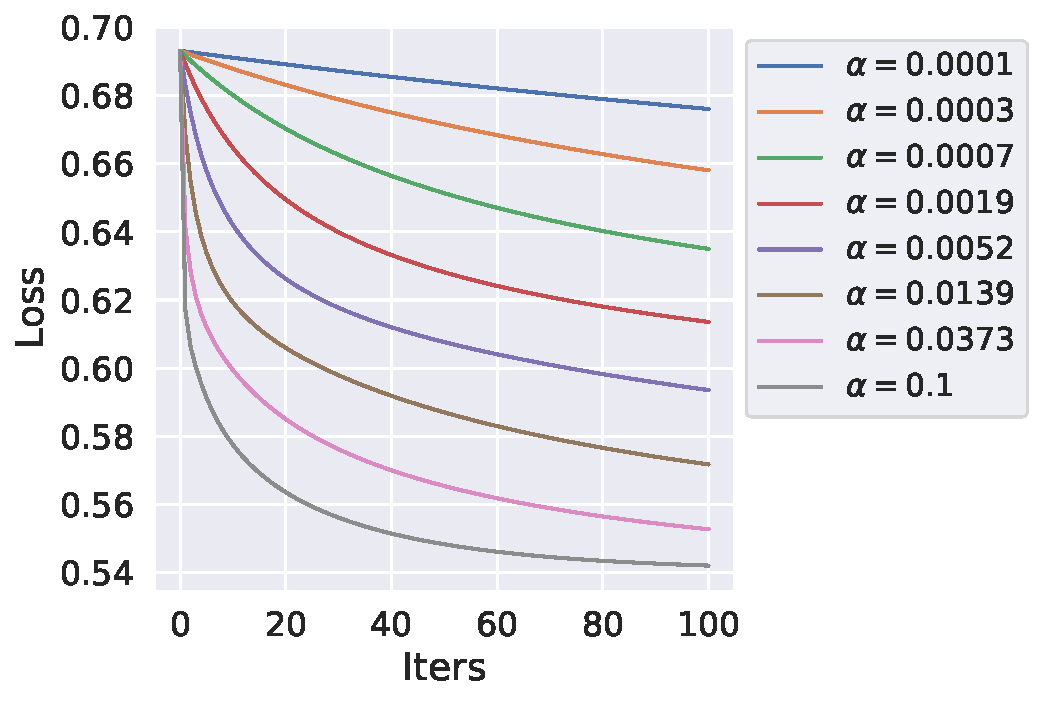
\includegraphics[width=\linewidth]{./experiment1/alpha/gd_loss__iters.pdf}
            \caption{}
        \end{subfigure}%
        \begin{subfigure}{.5\textwidth}
            \centering
            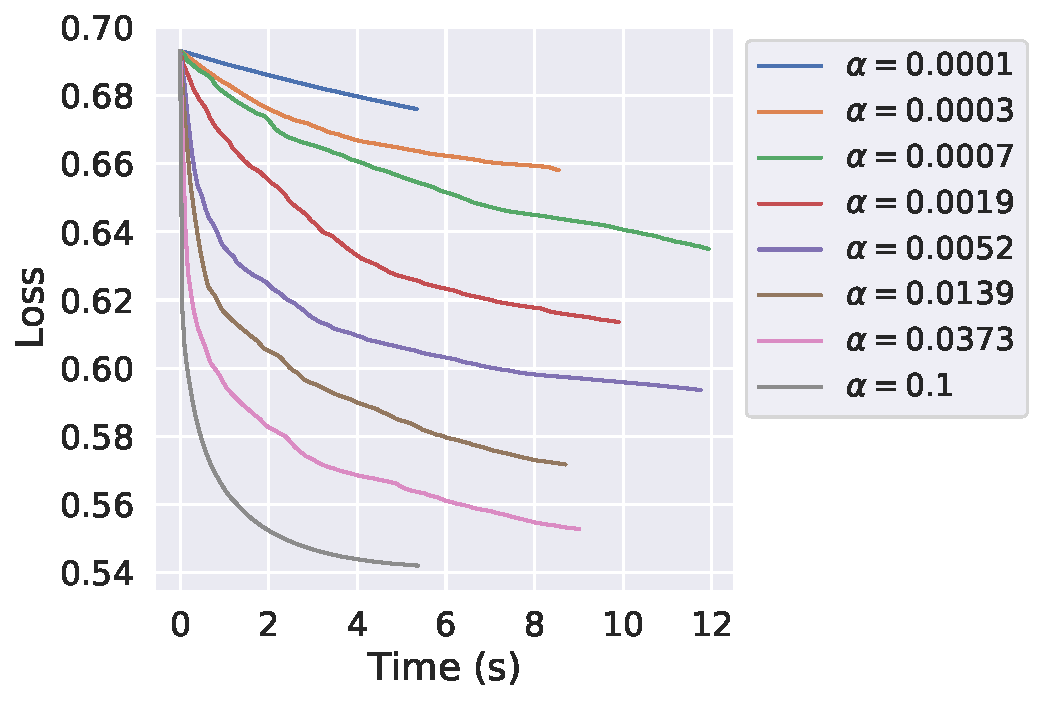
\includegraphics[width=\linewidth]{./experiment1/alpha/gd_loss_time.pdf}
            \caption{}
        \end{subfigure}
    \caption{}
	\end{figure*}\label{eq:exp1_fig1}
	Все графики зависимости от времени и итераций очень похожи друг на друга, поэтому в зависимости от потребностей в дальнейшем будут использоваться как графики от итераций так и графики от времени, а остальные будут помещены в {\bfseries Приложении А}. Из рис.\ref{eq:exp1_fig1} видно, что чем меньше $\alpha$ тем медленнее сходится к минимуму итерационный процесс, ему необходимо больше шагов итераций, так как темп обучения слишком мал. Впрочем, и слишком большие значения $\alpha$ не способствуют хорошей оптимизации (см. рис. \ref{eq:exp1_fig2}).
	\begin{figure}[h]
		
		\centering{
		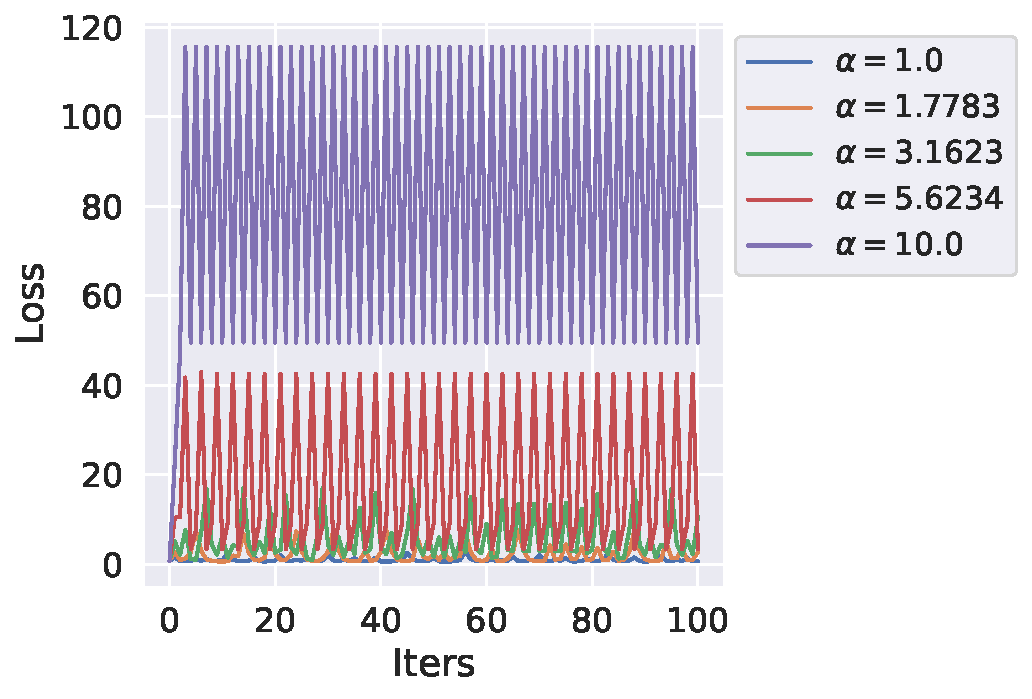
\includegraphics[width=0.8\textwidth]{./experiment1/alpha/gd_loss__iters_big_alphas.pdf}
		}
		\caption{}
		\label{eq:exp1_fig2}
	\end{figure}
	В результате выбора больших $\alpha \gtrapprox\!\!1.0$ уже наблюдается сильная осцилляция. При дальнейшем увеличение градиентный спуск на каждой итерации будет осциллировать около точки минимума(причем из графика видно, что при $\alpha = 10$ оцилляция уже происходит в области другой точки минимума). 
	Отрицательные значения  $\alpha$ бессмысленны, так как мы решаем задачу минимизации, а значит, нам нужен антиградиет, то есть градиент со знаком минус.
    %\newsavebox{\myimage}
    \begin{figure*}[h]
        \begin{subfigure}{.5\textwidth}
            \centering
            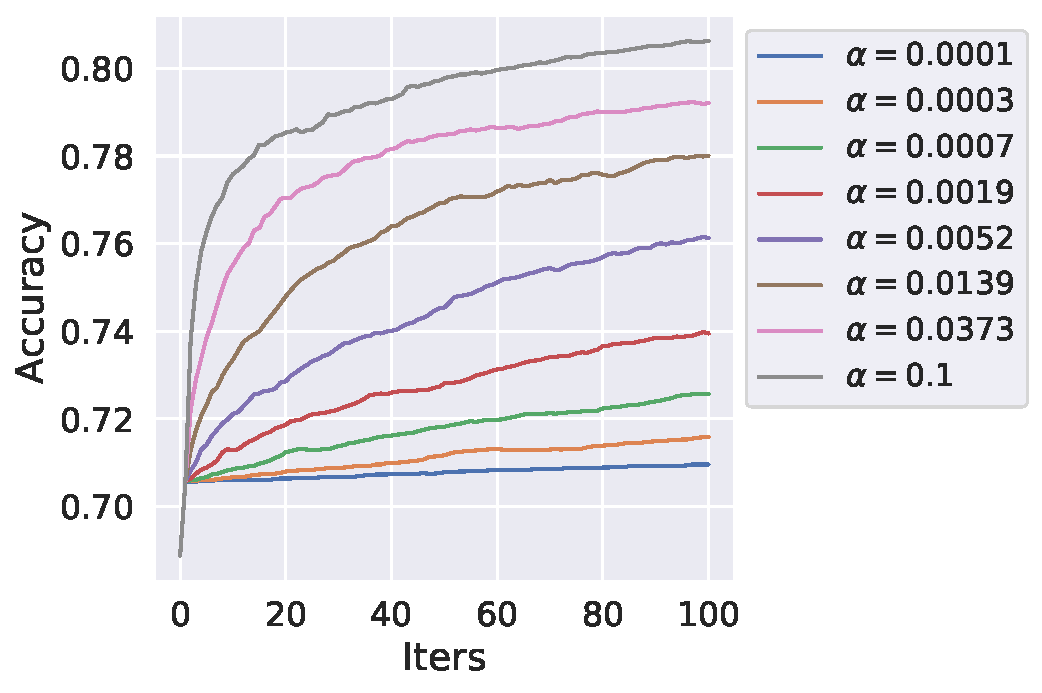
\includegraphics[width=\linewidth]{./experiment1/alpha/gd_acc_iters.pdf}
            \caption{}
        \end{subfigure}%
        \begin{subfigure}{.5\textwidth}
            \centering
            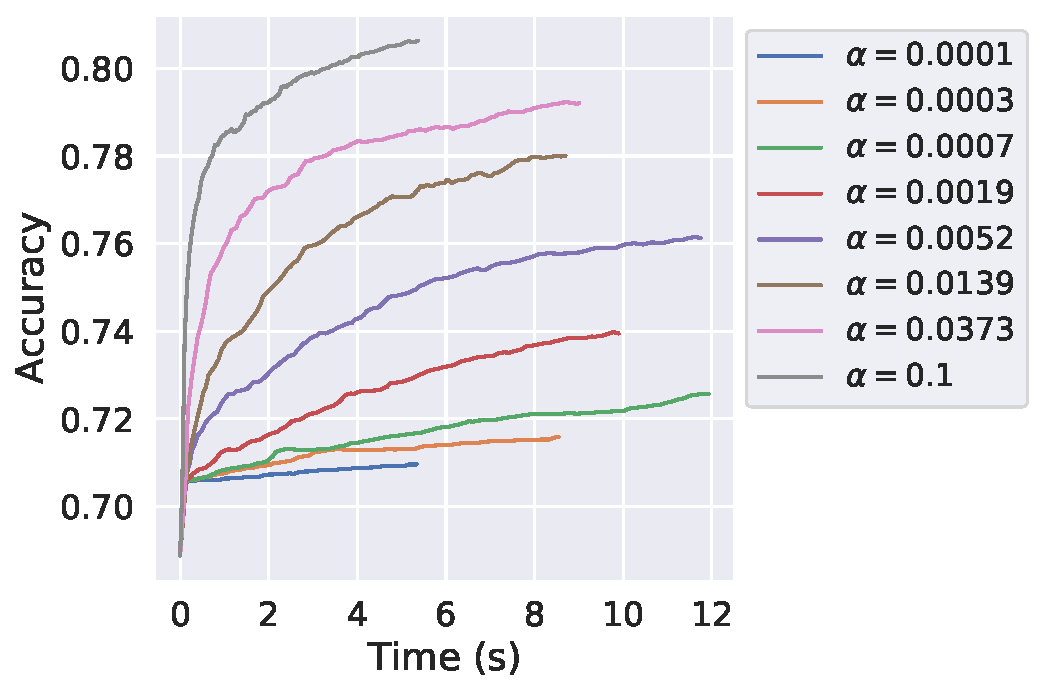
\includegraphics[width=\linewidth]{./experiment1/alpha/gd_acc_time.pdf}
            \caption{}
        \end{subfigure}
    \caption{}
    \label{eq:exp1_fig3}
	\end{figure*}
	Как видим из рис.\ref{eq:exp1_fig3} c увеличением $\alpha$ (при достаточно малых $\alpha$) быстрее достигается лучший accuracy. 
	
	\item{\bfseries  Выбор $\beta$}
	
	Теперь фиксируем $\alpha = 0.1$. При этом $\omega_0$ оставим той же. Будем перебирать по логарифмической сетке параметры $\beta$ 
    \begin{figure*}[h]
        \begin{subfigure}{.5\textwidth}
            \centering
            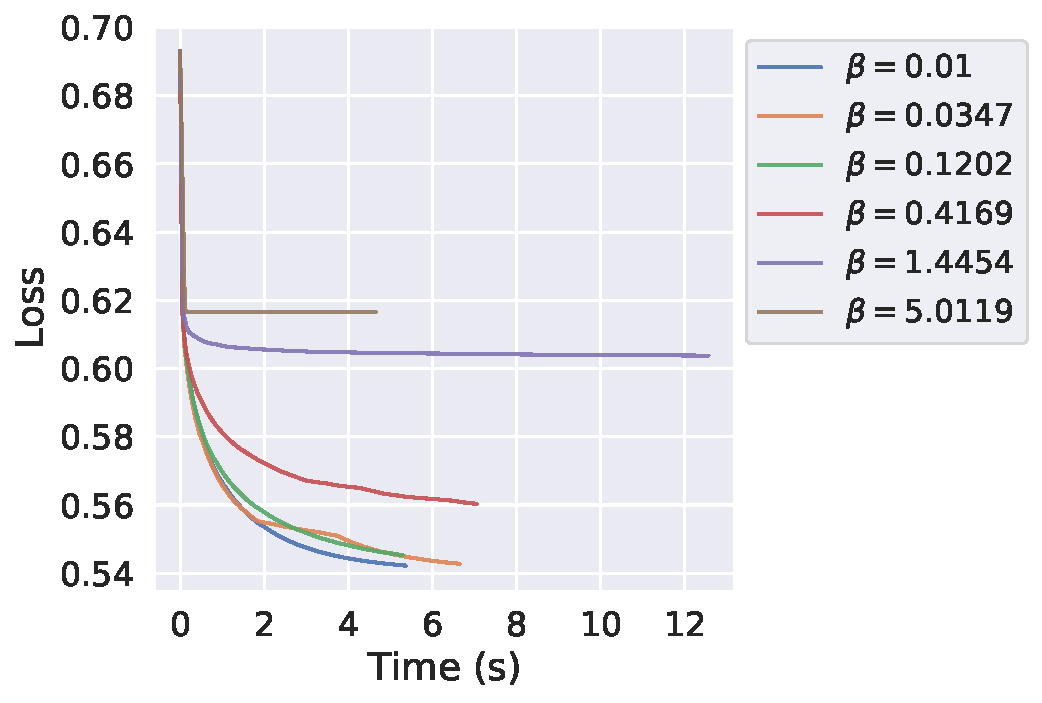
\includegraphics[width=\linewidth]{./experiment1/beta/gd_loss_time.pdf}
            \caption{}
        \end{subfigure}%
        \begin{subfigure}{.5\textwidth}
            \centering
            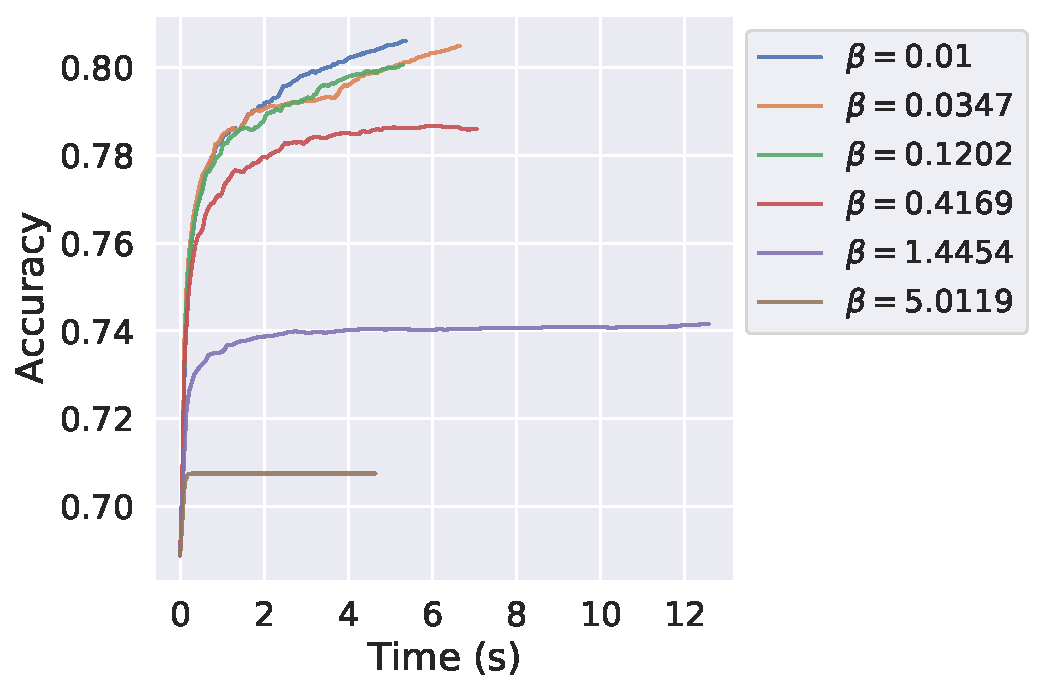
\includegraphics[width=\linewidth]{./experiment1/beta/gd_acc_time.pdf}
            \caption{}
        \end{subfigure}
    \caption{}
    \label{eq:exp1_fig4}
	\end{figure*}
	
	Из графика (рис.\ref{eq:exp1_fig4}) видно, что с уменьшением $\beta$ оптимизационная задача быстрее сходится к минимуму. При слишком больших $\beta\gtrapprox\!\!5$ алгоритм очень быстро закончит работать, поскольку из-за маленьких темпов обучения $\omega_k$(см. (\ref{grad})) будет не значительно меняться. С учетом гладкости функционала (см. Теоретическую часть) и его значения будут мало изменяться, следовательно условие останова цикла ($|Q(w_{k+1}) - Q(w_{k})| < tolerance$) будет быстро достигнуто и функция плохо решит оптимизационную задачу.

	Из рис.\ref{eq:exp1_fig4} следуют те же выводы, что и в случае с $\alpha$: c уменьшением $\beta$ оптимальная точность быстрее достигается

	\item{\bfseries  Выбор $\omega_0$}
	
	Фиксируем $\alpha = 0.1$, $\beta = 0.01$. Переберем $\omega_0$(см рис.\ref{eq:exp1_fig7}).
	\begin{figure}[h]		
		\centering{
		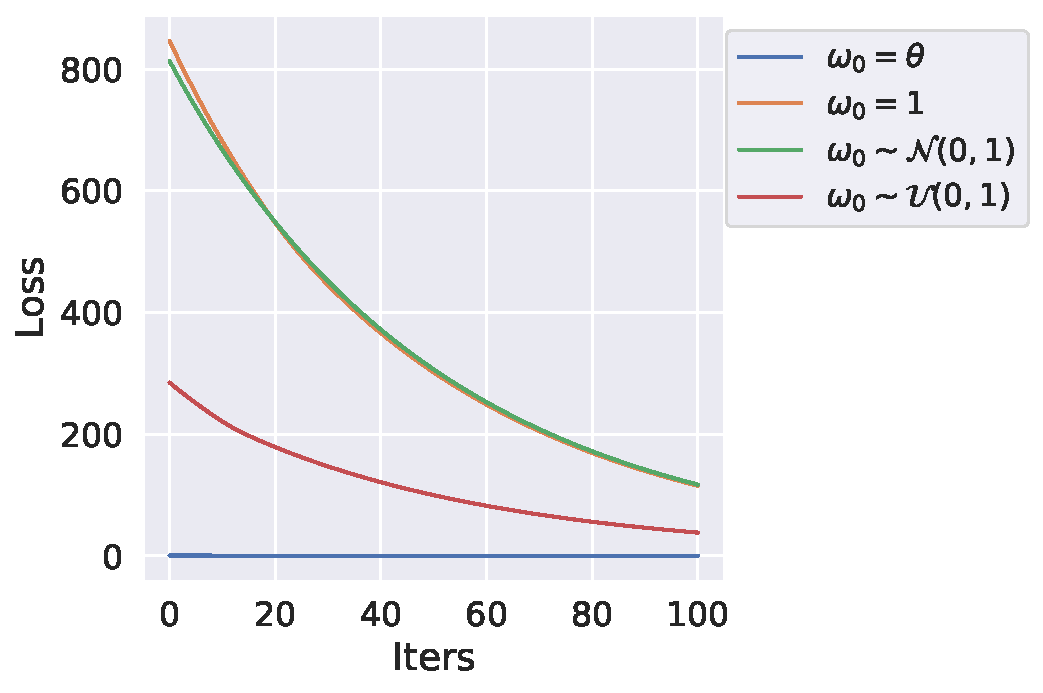
\includegraphics[width=0.8\textwidth]{./experiment1/w_0/gd_loss_iters.pdf}
		}
		\caption{}
		\label{eq:exp1_fig7}
	\end{figure}

	Некоторые пояснения:
	\begin{itemize}
		\item $\mathcal{N}$ - нормальное распределение
		\item $\mathcal{U}$ - равномерное распределение
	\end{itemize}
	Из графика (см. рис.\ref{eq:exp1_fig7}) видно, что с увеличением нормы $\omega_0$ значение функции потерь принимает большие значения. Лучшим вариантом будет взять $\omega_0 = 0$, тогда будет тратиться меньшее количество итераций на минимизацию, так как иначе сначала уйдет большое количество итераций на уменьшение больших значений функционала, а потом проблема возникнет с шагом (см. \ref{step}), так как он уже будет мал и значения функционала будут незначительно изменяться.\\
	Теперь посмотрим на точность при различных $\omega_0$ (см. рис. \ref{eq:exp1_fig8})
	\begin{figure}[h]		
		\centering{
		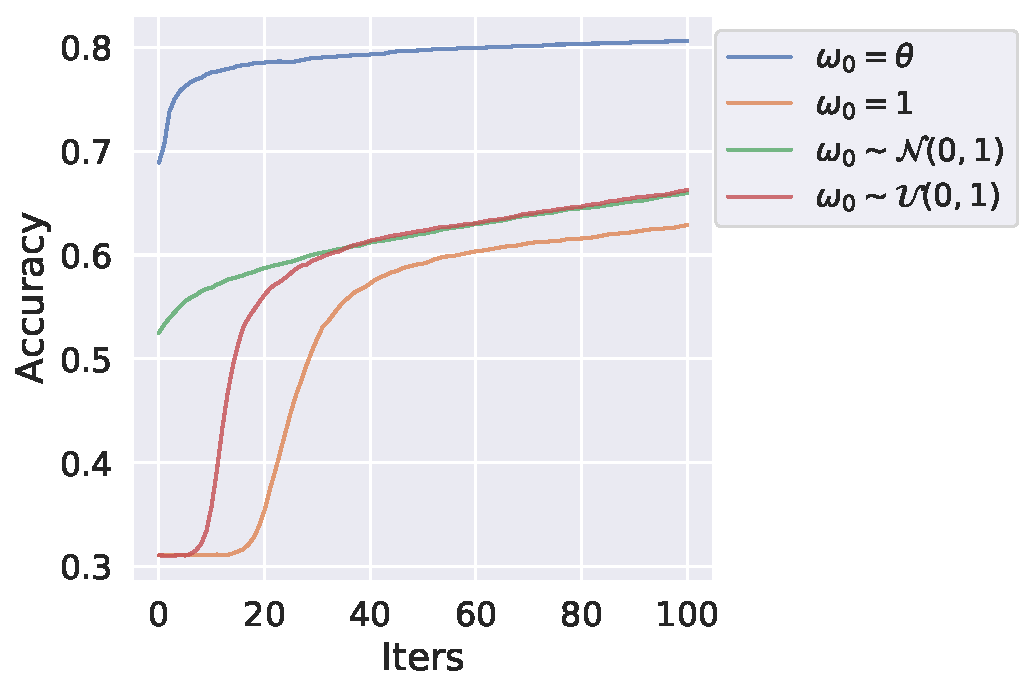
\includegraphics[width=0.8\textwidth]{./experiment1/w_0/gd_acc_iters.pdf}
		}
		\caption{}
		\label{eq:exp1_fig8}
	\end{figure}
\end{enumerate}
Точность также показывает правильность выбора начального приближения равного нулю.
\subsubsection{Выводы эксперимента}
Для градиентного спуска оптимальным будет следующий выбор параметров:
\begin{itemize}
	\item $\alpha \lessapprox\!1.0$
	\item $\beta \lessapprox\!0.15$
	\item $w = 0$, $0 \in \mathbb{R}^D$
\end{itemize}


\subsection{Эксперимент 2. Анализ оптимальных  параметров для SGD.}
\subsubsection{Дизайн эксперимента}
В ходе данного эксперимента исследовались параметры для SGD. Дизайн эксперимента полностью повторяет предыдущий эксперимент за исключением того факта, что к параметрам из предыдущего эксперимента добавился размер батча  ({\itshape batch\_size}). 
\subsubsection{Результаты эксперимента}
Сразу же заметим, что зависимость графиков от времени и от эпох очень похожи, поэтому все графики будут находиться в  {\bfseries Приложении Б}, а здесь же используются только необходимые.
\begin{enumerate}
	\item {\bfseries  Выбор $\alpha$}
	
	Фиксируем $\beta = 1$, $\omega_0 = 0 \in \mathbb{R}^D$, $batch\_size=10000$ и по логарифмической сетке рассмотрим различные параметры $\alpha$ (см. рис.\ref{eq:exp2_fig1}):
    %\newsavebox{\myimage}
    \begin{figure*}[h]
        \begin{subfigure}{.5\textwidth}
            \centering
            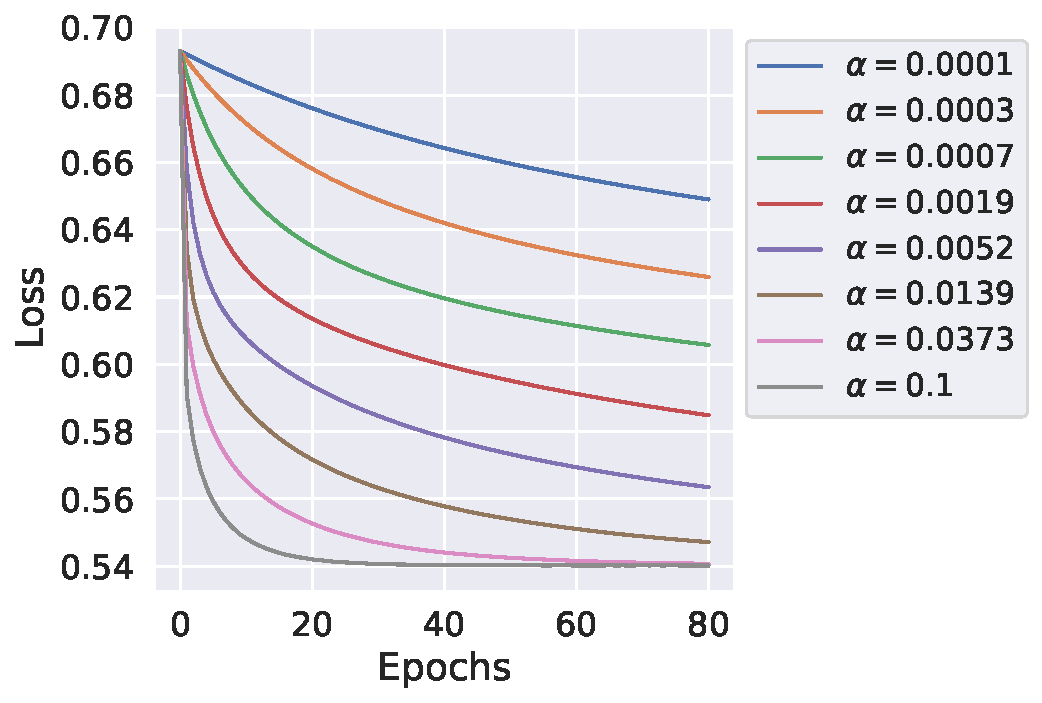
\includegraphics[width=\linewidth]{./experiment2/alpha/sgd_loss__iters.pdf}
            \caption{}
        \end{subfigure}%
        \begin{subfigure}{.5\textwidth}
            \centering
            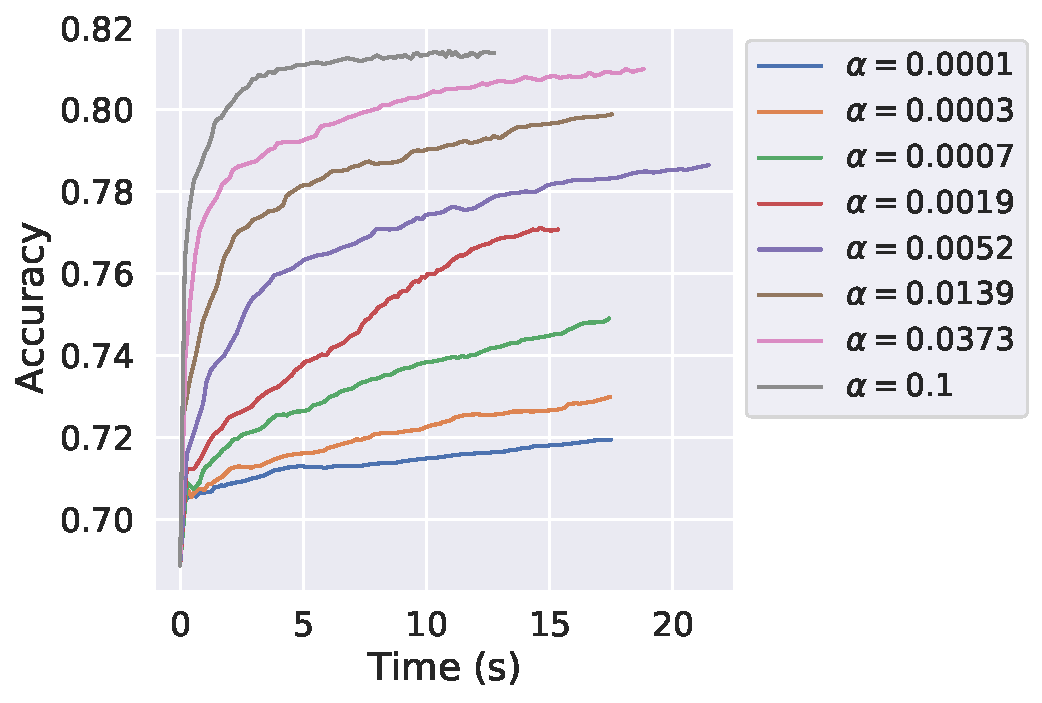
\includegraphics[width=\linewidth]{./experiment2/alpha/sgd_acc_time.pdf}
            \caption{}
        \end{subfigure}
    \caption{}\label{eq:exp2_fig1}
	\end{figure*}
	Из графика (см. рис.\ref{eq:exp2_fig1}) следуют точно такие же выводы как и в случае градиентного спуска, то есть при увеличении $\alpha$ (не больше~1) функция потерь быстрее стремиться к минимуму. При больших $\alpha$ уже видна осцилляция, а при дальнейшем увеличении задача минимизации уже не разрешима (см. {\bfseries Приложение Б}).

	Посмотрим на accuracy. Как видно из рис. \ref{eq:exp2_fig1} на валидационной выборке точность наилучшая при $\alpha=0.1$, при этом время работы при различных значениях данного параметра почти одинаково

	\item {\bfseries  Выбор $\beta$}
	
	Фиксируем $\alpha = 0.1$, $\omega_0 = 0 \in \mathbb{R}^D$, $batch\_size=10000$ и по логарифмической сетке рассмотрим различные параметры $\beta$ (см. рис.\ref{eq:exp2_fig2}):
	%\newsavebox{\myimage}
    \begin{figure*}[h]
        \begin{subfigure}{.5\textwidth}
            \centering
            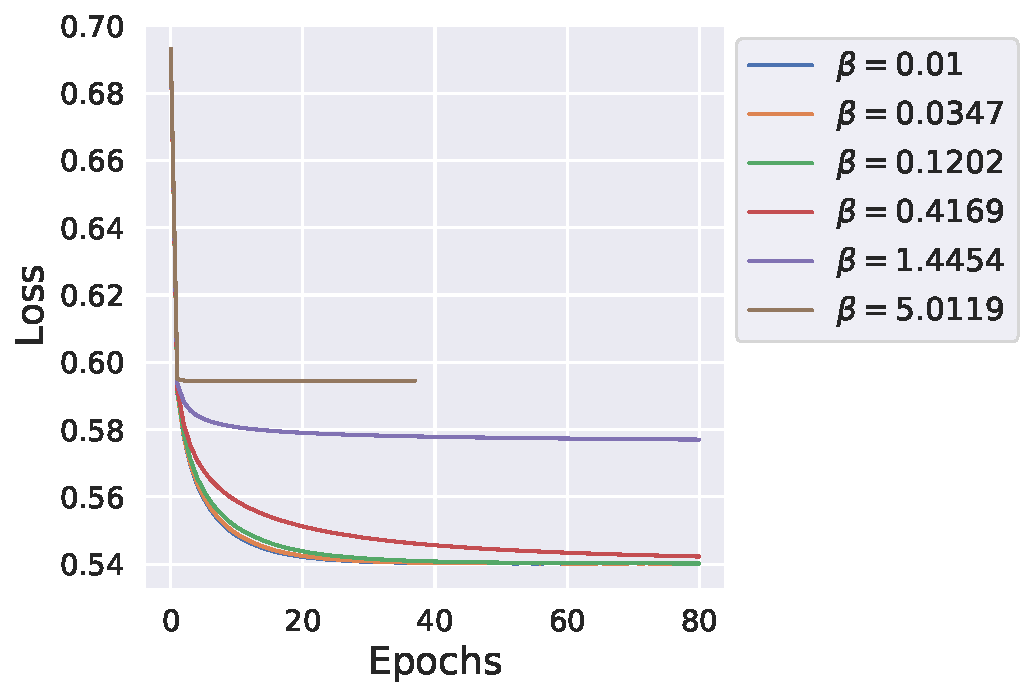
\includegraphics[width=\linewidth]{./experiment2/beta/sgd_loss__iters.pdf}
            \caption{}
        \end{subfigure}%
        \begin{subfigure}{.5\textwidth}
            \centering
            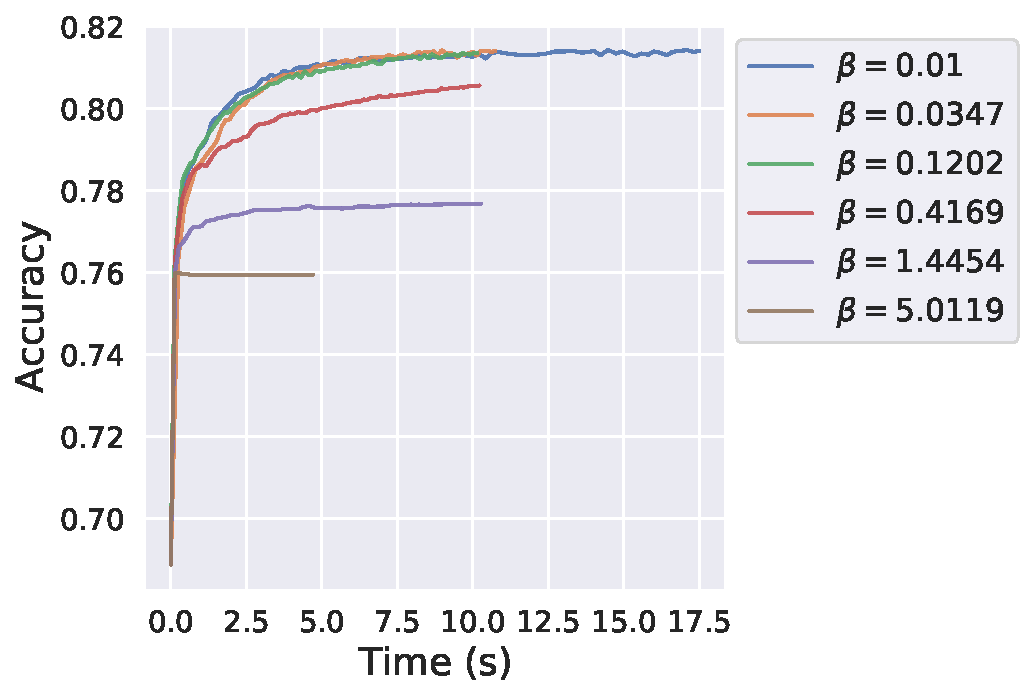
\includegraphics[width=\linewidth]{./experiment2/beta/sgd_acc_time.pdf}
            \caption{}
        \end{subfigure}
    \caption{}\label{eq:exp2_fig2}
    \end{figure*}
	Видно (см. рис.\ref{eq:exp2_fig2}), что тут такая же зависимость как и в случае градиентного спуска, то есть при уменьшении $\beta$ функция потерь быстрее стремиться к минимуму. При больших $\beta$ быстро выходит на плато и соответственно за короткое время достигает условия останова, о котором упомяналось выше.

	Исследуем accuracy.
	Наилучшим оказался $\beta=0.0347$ ({$accuracy =~0.8141$}), при этом при $\beta \lessapprox\!0.15$  {\itshape accuracy} тоже весьма хороший $\approx\!0.813$.

	\item {\bfseries  Выбор $\omega_0$}
	
	Фиксируем $\alpha = 0.1$, $\beta = 0.0347$, $batch\_size=10000$ и рассмотрим различные параметры $\omega_0$ (см. рис.\ref{eq:exp2_fig3}, рис.\ref{eq:exp2_fig4}):
	\begin{figure}[h]
		\centering{
		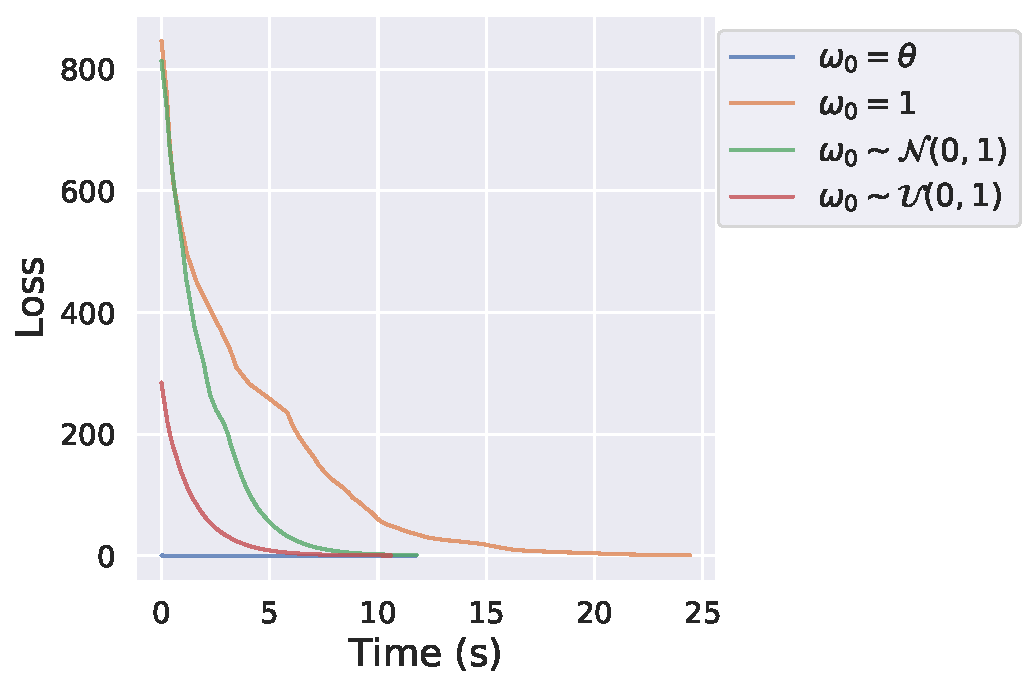
\includegraphics[width=0.7\textwidth]{./experiment2/w_0/sgd_loss_time.pdf}
		}
		\caption{}
		\label{eq:exp2_fig3}
	\end{figure}
	
	\begin{figure}[h]
		\centering{
		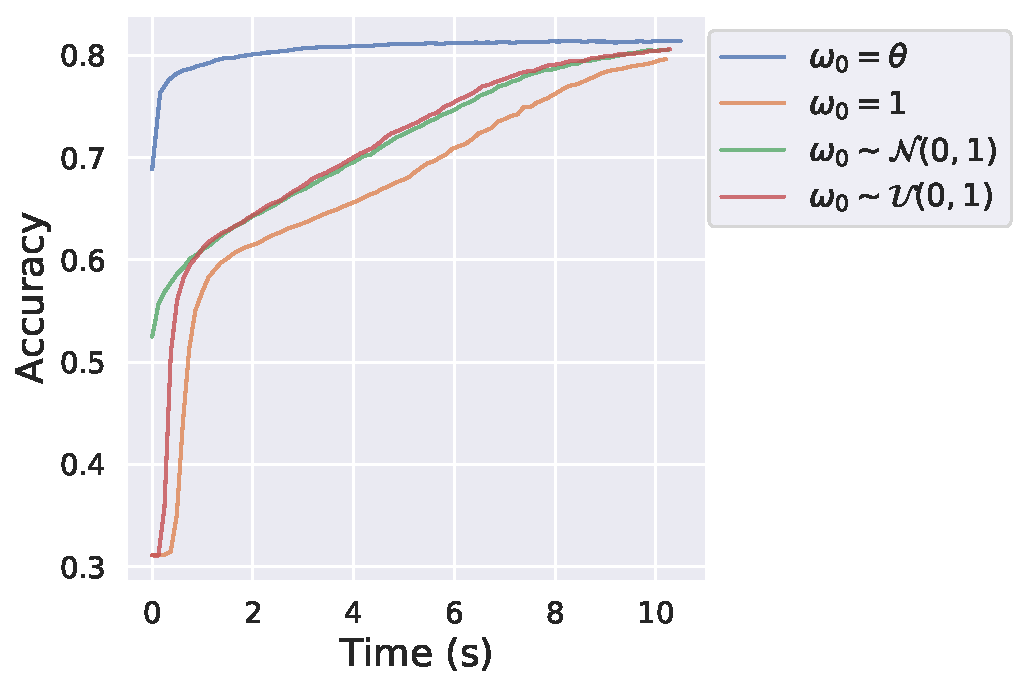
\includegraphics[width=0.7\textwidth]{./experiment2/w_0/sgd_acc_time.pdf}
		}
		\caption{}
		\label{eq:exp2_fig4}
	\end{figure}
	По-прежнему лучшим начальным приближением является $\omega_0=0$. Из необычного несложно заметить, что в отличие от эксперимента 1\footnote{В эксперименте 1 {\itshape accuracy} для $\omega_0 \neq 0$ равен $\approx 0.65$} в этом $accuracy$ для всех рассмотренных случаев значительно ближе к наилучшей оценке минимума для $\omega_0 = 0$ и достигается за меньшее количество времени чем для GD.

	\item {\bfseries  Выбор $batch\_size$}
	
	Фиксируем $\alpha = 0.1$, $\beta = 0.0347$, $\omega_0=0$ и рассмотрим различные параметры batch\_size (см. рис.\ref{eq:exp2_fig5}):
	\begin{figure*}[h]
        \begin{subfigure}{.5\textwidth}
            \centering
            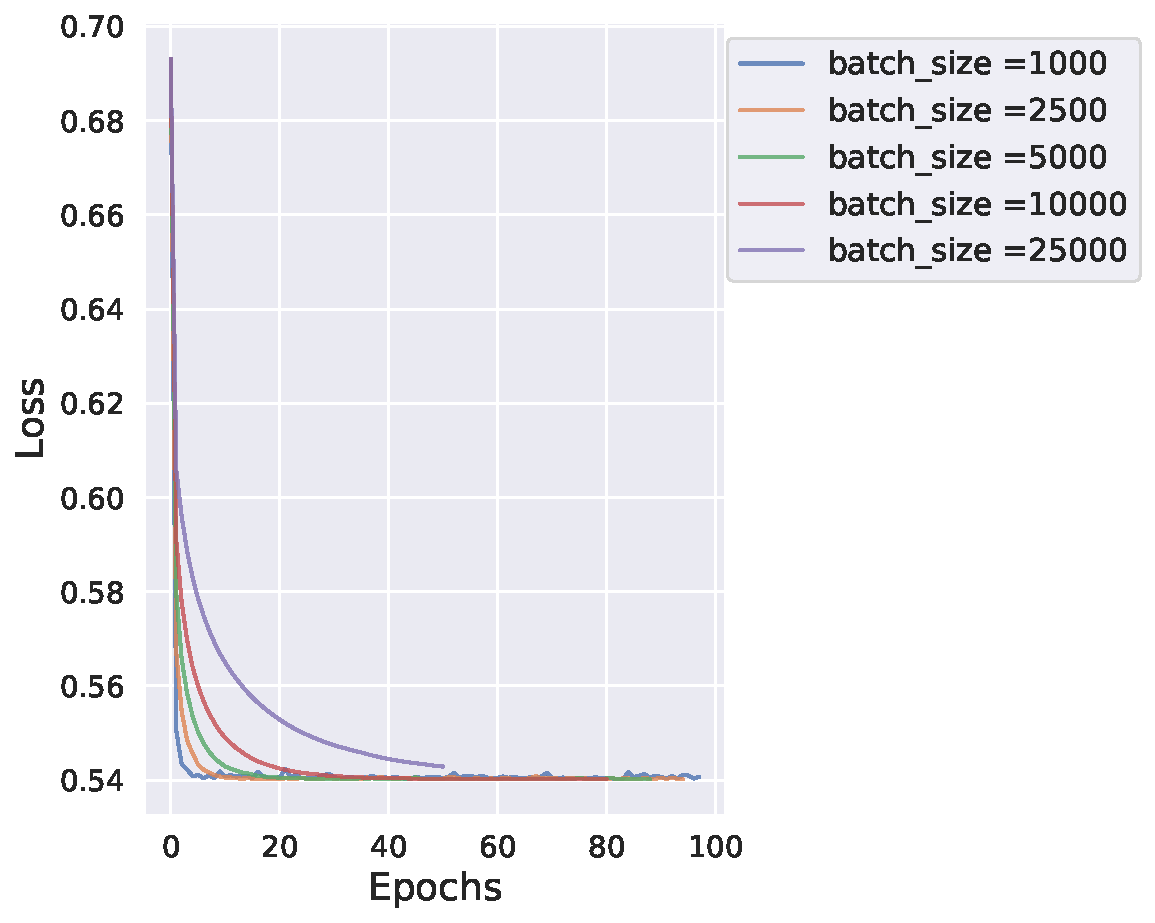
\includegraphics[width=\linewidth]{./experiment2/batch_size/sgd_loss_iters.pdf}
            \caption{}
        \end{subfigure}%
        \begin{subfigure}{.5\textwidth}
            \centering
            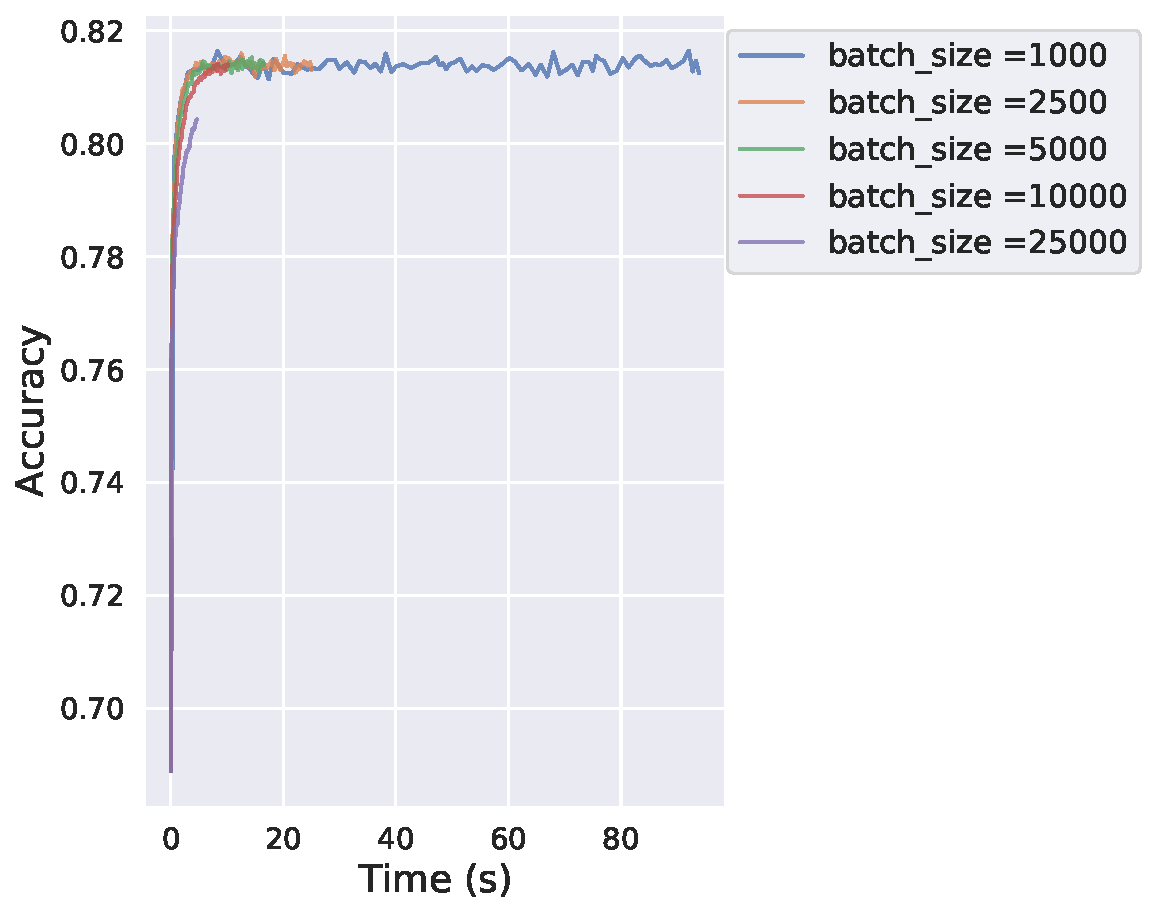
\includegraphics[width=\linewidth]{./experiment2/batch_size/sgd_acc_time.pdf}
            \caption{}
        \end{subfigure}
    \caption{}\label{eq:exp2_fig5}
    \end{figure*}
	Проанализировав рис.\ref{eq:exp2_fig5}, можно заметить что чем меньше размер батча тем меньше эпох, а значит, меньше потраченного времени нужно для достаточно неплохих оценок минимума функционала. Также видно, что с уменьшением батча увеличивается осцилляция. Хотя наилучшая точность на валидационной выборке была достигнута с $batch\_size = 1000$    ($accuracy = 0.8145$), в дальнейшем будет использоваться $batch\_size = 10000 $ ($accuracy = 0.8141$), поскольку он оптимален по нескольким параметрам: время (в $\approx\!8$  раз быстрее работает чем с $batch\_size = 1000$), $accuracy$ и устойчивость(меньше осцилляций, а значит при одних и тех же значениях метод будет получать более устойчивые оценки точности, чем с меньшими значениями размера)
\newpage
\subsubsection{Выводы эксперимента}
Для стохастического градиентного спуска оптимальным будет следующий выбор параметров:
\begin{itemize}
	\item $\alpha \lessapprox\!1.0$
	\item $\beta \lessapprox\!0.15$
	\item $w = 0$, $0 \in \mathbb{R}^D$
	\item $batch\_size \leq 10000$
\end{itemize}
\end{enumerate}

\subsection{Эксперимент 3. Сравнение SGD и GD.}
\subsubsection{Дизайн эксперимента}
Для сравнения двух методов бралось множество оптимальных параметров, подобранных в предыдущих экспериментах, а именно:
\begin{itemize}
	\item Для GD:
	\begin{enumerate}
		\item $\alpha = 0.1$
		\item  $\beta = 0.01$
		\item  $\omega_0 = 0 \in \mathbb{R}^D$
	\end{enumerate}
	\item Для SGD:
	\begin{enumerate}
		\item $\alpha = 0.1$
		\item  $\beta = 0.0347$
		\item  $\omega_0 = 0 \in \mathbb{R}^D$
		\item  $batch\_size = 10000 $
	\end{enumerate}
\end{itemize}

Далее исследовались методы GD и SGD с данными параметрами по $accuracy$, времени и значению функции потерь.

\subsubsection{Результаты эксперимента}
\begin{figure*}[h]
	\begin{subfigure}{.5\textwidth}
		\centering
		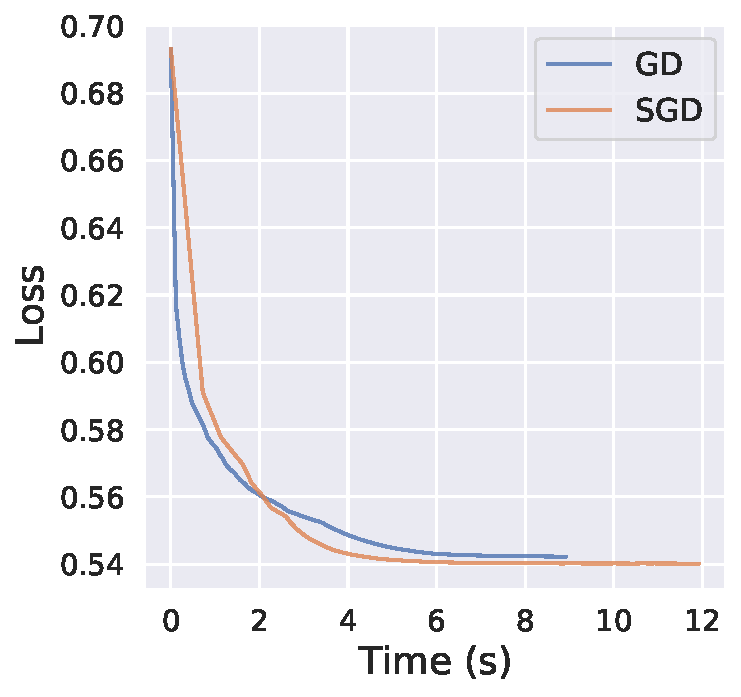
\includegraphics[width=\linewidth]{./experiment3/loss_time.pdf}
		\caption{}
	\end{subfigure}%
	\begin{subfigure}{.5\textwidth}
		\centering
		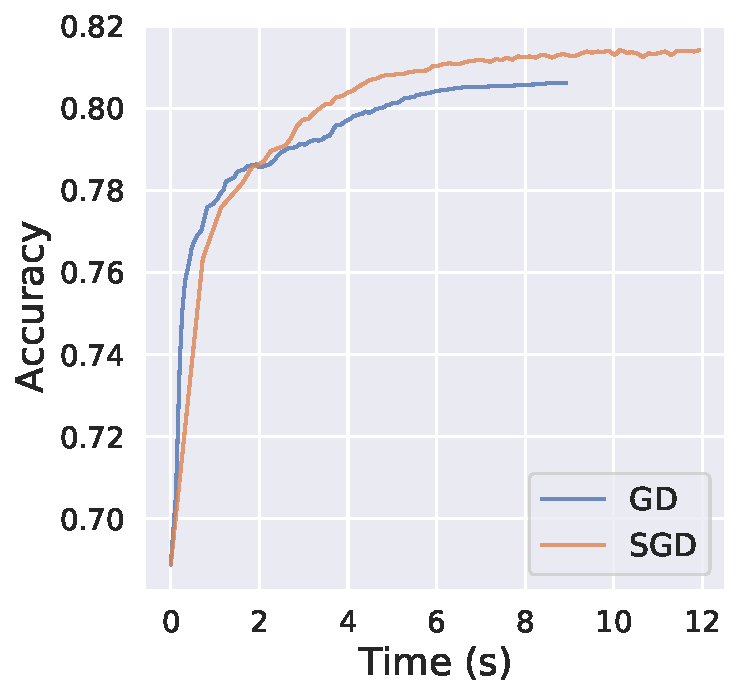
\includegraphics[width=\linewidth]{./experiment3/acc_time.pdf}
		\caption{}
	\end{subfigure}
\caption{}\label{eq:exp3_fig1}
\end{figure*}

\begin{tabular}{|c|c|c|c|}
	\hline
	\multicolumn{4}{|c|}{Сравнение методов}\\
	\hline
		Название  градиентного метода & Время (с)  & Лосс & $accuracy$ \\
	\hline
	  GD & 8.925143 &  0.542243 & 0.806100 \\
	\hline
	  SGD & 11.928005 & 0.540191 & 0.814100 \\
	\hline
\end{tabular}\\


Из рис.\ref{eq:exp3_fig1} и таблицы  видно, что по точности и качеству оптимизации с точки зрения близости к минимуму, а не времени качественно лучше стохастический градиентный спуск. Вычислительная сложность для GD будет $O(N*D*max\_iters)$, а для SGD $O(N*D*max\_iters* \lceil \frac{N}{batch\_size}\rceil)$\footnote{$max\_iters$ для SGD это количество эпох}, поэтому не удивительно, что работать SGD будет дольше.
\subsubsection{Выводы эксперимента}
По качеству наилучшим методом оказался SGD, но по времени он проигрывает GD. При этом с уменьшением размера батча время работы SGD будет увеличиваться обратно пропорционально.


\subsection{Эксперимент 4. Предобработка корпуса и ее влияние на качество модели.}
\subsubsection{Дизайн эксперимента}
В данном эксперименте использовались те же параметры, что и в предыдущем:
\begin{itemize}
	\item Для GD:
	\begin{enumerate}
		\item $\alpha = 0.1$
		\item  $\beta = 0.01$
		\item  $\omega_0 = 0 \in \mathbb{R}^D$
	\end{enumerate}
	\item Для SGD:
	\begin{enumerate}
		\item $\alpha = 0.1$
		\item  $\beta = 0.0347$
		\item  $\omega_0 = 0 \in \mathbb{R}^D$
		\item  $batch\_size = 10000 $
	\end{enumerate}
\end{itemize}
В этом эксперименте рассматривалось влияние на  время работы градиентного метода, $accuracy$, и размерность признакового пространства $D$ таких методов предобработки как:
\begin{itemize}
	\item лемматизация(сведение слово к начальной форме, к лемме). Пример:
	"write wrote written" \ $\rightarrow$ "write write write"
	\item удаление стоп-слов (предлоги, частицы и другие шумовые слова). Пример:
	"The Moscow is the best city" \ $\rightarrow$ "Moscow best city"
\end{itemize}
Для определения влияния обработки рассматривались время, $accuracy$, размер признакового пространства по выборке до обработки и те же самые параметры по выборке после обработки. Сравнение велось как для SGD, так и для GD.
\subsubsection{Результаты эксперимента}
\begin{tabular}{|c|c|c|c|}
	\hline
		& Время (с)  & Количество признаков & $accuracy$ \\
	\hline
		GD без обработки & 8.925143 &  16050 & 0.806100 \\
	\hline
		GD с обработкой & 5.081007 & 12964 & 0.820700 \\
	\hline
		SGD без обработки & 11.928005 &  16050 & 0.814100 \\
	\hline
		SGD с обработкой & 10.939810 & 12964 & 0.830700 \\
	\hline
\end{tabular}\\

Сразу заметим, что размерность признакового пространства сильно уменьшилась. Из-за уменьшения размерности пространства с учетом вычислительной сложности для GD и SGD, полученной выше в эксперименте 3, очевидно, уменьшится и время работы модели, что подтверждается значениями в таблице. Из таблицы также следует, что лемматизация и удаление стоп-слов способствует значительному улучшению точности: для GD на 7.52\% меньше ошибок (на $\approx 145$ меньше текстов-ошибок для валидационной выборки размера 10000), а для SGD на 8.92\% меньше ошибок (на $\approx 165$ меньше текстов-ошибок для валидационной выборки размера 10000). 
\subsubsection{Выводы эксперимента}
Предобработка корпуса с помощью лемматизации и последующего удаления стоп-слов дает не только выигрыш в памяти, но и позволяет улучшить модель по времени и точности.

\subsection{Эксперимент 5. Векторизация текстов. Выбор параметров min\_df и max\_df}
\subsubsection{Дизайн эксперимента}
Заданы: \\
\begin{itemize}
	\item Общие значения параметров, по которым идет перебор:
	\begin{enumerate}
		\item $min\_df = 0.00001, 0.0001, 0.01, 0.1, 0.3$
		\item  $max\_df = 0.1, 0.25, 0.35, 0.45, 0.55, 0.7$
	\end{enumerate}
	\item Для GD:
	\begin{enumerate}
		\item $\alpha = 0.1$
		\item  $\beta = 0.01$
		\item  $\omega_0 = 0 \in \mathbb{R}^D$
	\end{enumerate}
	\item Для SGD:
	\begin{enumerate}
		\item $\alpha = 0.1$
		\item  $\beta = 0.0347$
		\item  $\omega_0 = 0 \in \mathbb{R}^D$
		\item  $batch\_size = 10000 $
	\end{enumerate}
\end{itemize}

В данном эксперименте анализируется влияние на точность, время работы, размер признакового пространства различных методов векторизации текстов, параметров min\_df и  max\_df. В качестве методов векторизации будут рассмотрены два метода:
{\bf BagOfWords(BOW)}, основанный на подсчете количества повторений уникальных слов, и {\bf Tf-Idf}, основанный на подсчете количества повторений уникальных слов с поправкой на частоту встречаемости во всей коллекции текстов. После изучения векторизации, будет рассмотрен min\_df, а уже после того, как будет найден оптимальный min\_df будет изучен вопрос об оптимальном max\_df. Также стоит отметит, что в ходе этого эксперимента в качестве валидационной и обучающей выборки брались валидационноая и обучающую выборка, которая обсуждалась в самом начале раздела "Список экспериментов".
\subsubsection{Результаты эксперимента}
\begin{enumerate}
	\item {\bf BagOfWords и Tf-Idf}\\ \\
	\begin{tabular}{|c|c|c|c|c|}
		\hline
			Метод & Вид векторизации & Время (с)  & Количество признаков & $accuracy$ \\
		\hline
		\hline
			GD 
			& BOW & 7.759336 &  16050 &  0.806100\\ \cline{2-5}
			& Tf-Idf & 6.127796 & 16050 & 0.721500 \\
		\hline
			SGD 
			& BOW & 11.931548 &  16050 & 0.814100 \\ \cline{2-5}
			& Tf-Idf & 8.624678 & 16050 & 0.723900 \\
		\hline
	\end{tabular}\\

	Таблица выше была построена по предсказаниям на валидационной выборке.Заметим, что при данных методах векторизации размерность признакового пространства не изменяется. Время незначительно, но все же меньше в обоих случаях при использовании Tf-Idf. Что же касается $accuracy$, то, вероятно, в текстах часто можно встретить слова, например, "you"{}, "like"{}, которые, вообще говоря, присутствуют во многих текстах, а значит, будут иметь маленький вес в Tf-Idf. При этом количество этих слов сильно возрастает в токсичных текстах для сравнения человека с чем-то, поэтому хотелось бы, чтобы мы это как-то учитывали в модели, но из-за малых весов эта информация не будет почти учитываться. \\
	{\bfseriesПримеры: }
	\begin{itemize}
		\item "fuck you  you stupid american"
		\item "you are such a dickhead  you lesbian butch"
	\end{itemize}
	
	\item {\bf min\_df}\\ 
	
	\begin{figure*}[h]
        \begin{subfigure}{.5\textwidth}
            \centering
            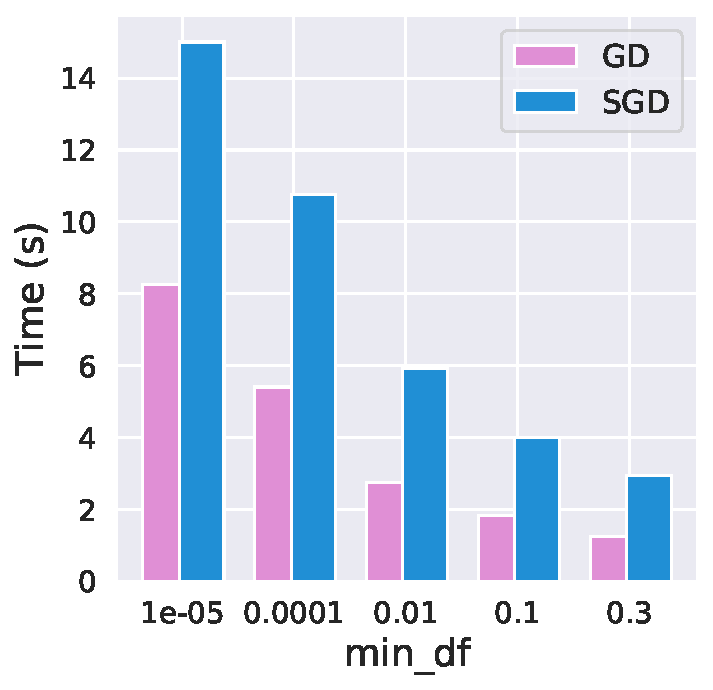
\includegraphics[width=0.9\linewidth]{./experiment5/mindf_time.pdf}
            \caption{}
        \end{subfigure}%
        \begin{subfigure}{.5\textwidth}
            \centering
            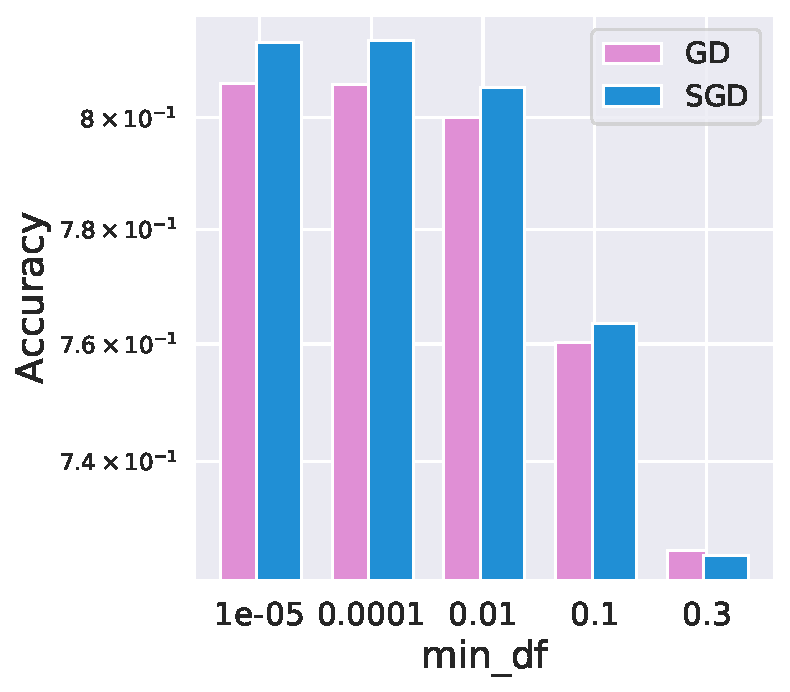
\includegraphics[width=\linewidth]{./experiment5/mindf_acc.pdf}
            \caption{}
        \end{subfigure}
    \caption{}\label{eq:exp5_fig1}
    \end{figure*}
	Из рис.\ref{eq:exp5_fig1} видно, что чем меньше  значение 
	$min\_df$, тем GD и SGD больше тратят времени на минимизацию функционала $Q(w)$, это неудивительно, так как размер признакового пространства увеличивается (см. таблицу ниже)\footnote{Оценки вычислительной сложности GD и SGD были даны выше в эксперименте 3}. Также из графика зависимости $accuracy$ от $min\_df$ видно, что при $min\_df\lessapprox 0.0001$ точность примерно такая же как и при $min\_df =0.0001$ (при $min\_df = 0.0001$ она даже выше чем при $min\_df =10^{-5}$ : 0.8141 против 0.8137), а при $min\_df \gtrapprox 0.0001$ уже начинается падение точности. Видимо, при больших $min\_df$ слишком много полезных признаков пропадает, так как признак(слово) выкидывается тогда, когда частота его встречаемости во всех текстах меньше заданного значения $min\_df$.

	\item {\bf max\_df}\\ 
	
	Фиксируем теперь оптимальный $min\_df = 0.0001$. Тут со временем ситуация такая же как и у $min\_df$ с увеличением $max\_df$ увеличивается признаковое пространство (см. таблицу ниже и рис.\ref{eq:exp5_fig3}), поэтому и время увеличивается. 
	\begin{figure*}[h]
        \begin{subfigure}{.5\textwidth}
            \centering
            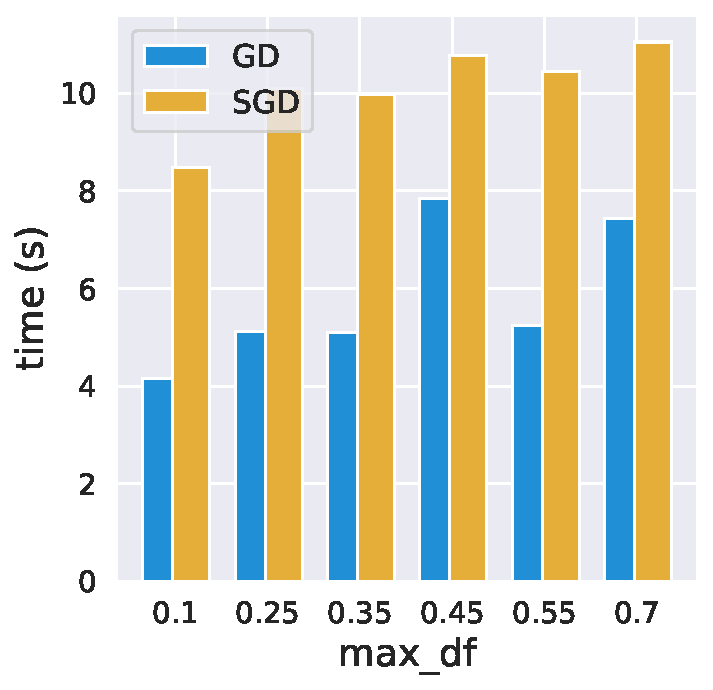
\includegraphics[width=0.9\linewidth]{./experiment5/maxdf_time.pdf}
            \caption{}
        \end{subfigure}
        \begin{subfigure}{.5\textwidth}
            \centering
            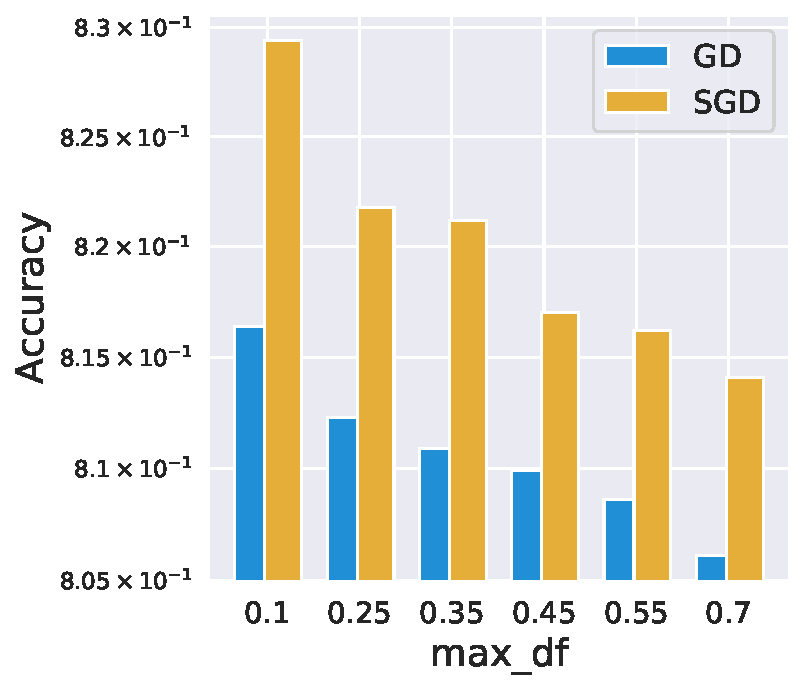
\includegraphics[width=\linewidth]{./experiment5/maxdf_acc.pdf}
            \caption{}
        \end{subfigure}
    \caption{}\label{eq:exp5_fig3}
    \end{figure*}
	Также нетрудно заметить, что $max\_df$ c увеличением своего значения лишь понижает точность алгоритма.
\end{enumerate}
\begin{center}
	{\bf Таблица зависимости количества признаков от значений min\_df и max\_df}\\
\end{center}

\begin{tabular}{|c|c|c||}
	\hline
		Параметр & Значение параметра & Количество признаков \\
	\hline
	\hline
		$min\_df$
		& 0.00001 & 89368	\\ \cline{2-3}
		& 0.0001 & 16050	\\\cline{2-3}
		& 0.01 & 568		\\\cline{2-3}
		& 0.1 & 55			\\\cline{2-3}
		& 0.3&  11			\\\cline{2-3}
	\hline
	\hline
	\hline
		$max\_df$
		& 0.1 & 15995		\\ \cline{2-3}
		& 0.25 & 16034		\\\cline{2-3}
		& 0.35 & 16041		\\\cline{2-3}
		& 0.45 & 16046		\\\cline{2-3}
		& 0.55&  16048		\\\cline{2-3}
		& 0.7&  16050		\\\cline{2-3}
	\hline
\end{tabular}\\
\subsubsection{Выводы эксперимента}
\begin{itemize}
	\item Tf-Idf плохо использовать для задачи определения токсичности комментария, так как он может давать малые веса часто употребляемым словам, которые в токсичных текстах чаще обычного встречаются
	\item Из расмотренных параметров наилучшими являются $min\_df =~0.0001$ и $max\_df=0.1$ 
\end{itemize}
\subsection{Эксперимент 6.  Лучший алгоритм. Анализ ошибок алгоритма.}
\subsubsection{Дизайн эксперимента}
В ходе данного эксперимента брались лучшие параметры, подобранные на предыдущих шагах и лучший из разобранных алгоритмов (SGD):
\begin{enumerate}
	\item $\alpha = 0.1$
	\item  $\beta = 0.0347$
	\item  $\omega_0 = 0 \in \mathbb{R}^D$
	\item  $batch\_size = 10000 $
	\item Текст подвергался лемматизации и выкидыванию стоп-слов
	\item Использовалась модель векторизации BagOfWords
	\item $min\_df = 0.0001$
	\item $max\_df = 0.1$
	\item $max\_iters = 1000$ (для увеличения точности)
\end{enumerate}
В этом эксперименте в качестве обучающей и тестовой были взяты исходные данные, то есть никакого деления на валидационную выборку уже не происходило. После обучения на обучающей выборке была построена и проанализирована матрица ошибок предсказания на тестовых ответах. Также были разобраны типичные ошибки алгоритма на примерах.
\newpage
\subsubsection{Результаты эксперимента}
\begin{figure}[h]
	\caption{\centering Матрица ошибок}
	\centering{
	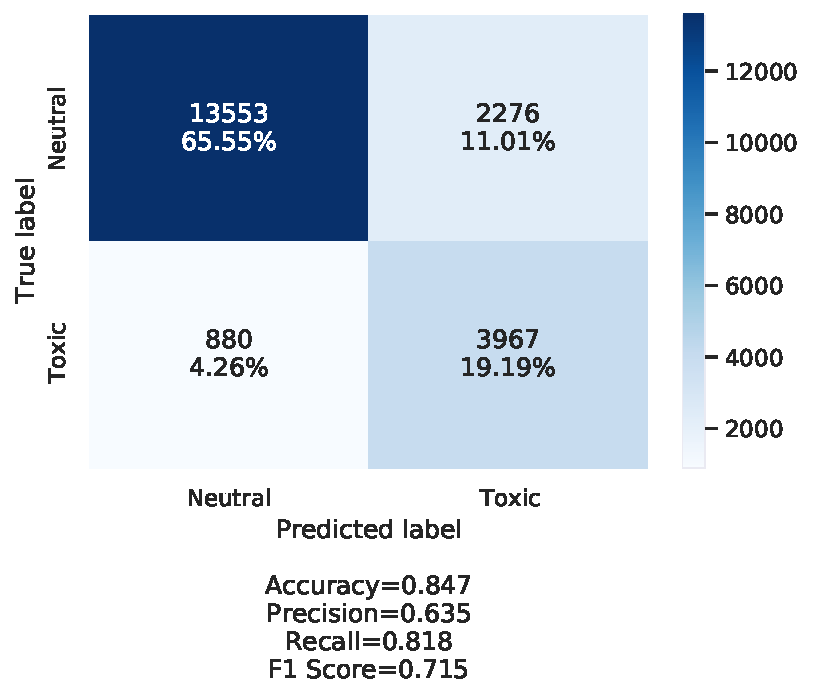
\includegraphics[width=0.7\linewidth]{conf_m.pdf}
	}
	\label{eq:confm}
\end{figure}
Как видим из рис.\ref{eq:confm} следует, что модель хорошо классифицирует
тексты, однако все же делает ошибки и чаще всего при классификации нейтральных текстов как токсичных. Рассмотри примеры текстов, на которых алгоритм чаще всего ошибается:\\
\begin{itemize}
	\item {\itshape "i think the origin of sagging has his roots in that human stupidity has no limits"{}, "alex  think again  mr  obama is the us  president  what about putin and his background  worse than an ass"{}} \\-- эти предложения были классифицированы, как нейтральные, хотя не являются такими. Вероятно, это происходит из-за того, что в этих текстах большая часть слов по-отдельности (кроме "stupidity" и "ass") это вполне обычные слова, употребляемые и в нейтральных текстах. \\
	\item "she looks like a horse" {} -- {}"horse" \ редко употребляется в качестве оскорбления, поэтому не верно классифицирован как нейтральный 
	\item "f u c k e r c o m m i e"{} -- из-за того, что есть пробельные слова это предложение будет представлено в виде вектора букв, а не слова. Понятно, что модель будет давать плохое предсказание, так как буквы не слова.
	\item {\itshape "we got snow here in boston  too    flying home tomorrow is going to suck"{}, "racism in moby dick       was herman melville a racist   particularly chapter 42 of moby dick  melville expounds on the terrifying aspects of the color white  how white dominates other colors  and how the white race dominates other races   was moby dick  the white whale  a symbol of white superiority and pride   i was shocked when i read this statement from chapter 42 pg  163 norton   1967  speaking on whiteness  melville writes       and though this preeminence in it applies to the human race itself  giving the white man mastership over every dusky tribe"{}}\\- тексты неверно классифицированы как токсичные. Алгоритм, ошибается, поскольку,  модель не знает контекст, и ошибочно воспринимает такие слова как "suck"\  и "dick"\  в "moby dick"\  как токсичные.
\end{itemize}
\subsubsection{Выводы эксперимента}
Таким образом, в основном алгоритм ошибается, поскольку не знает контекста, хотя бывает и в следствие наличия в текстовых данных данных, которые с формальной точки зрения не являются текстами (то есть непустой последовательностью, состоящей из слов, а не букв)
\section{\huge Общие выводы}

В рамках проведенного исследования были достигнуты поставленные цели и решены сформулированные в начале исследования задачи. Особенно хотелось бы выделить следующие результаты:
\begin{itemize}
	\item в рамках нашей задачи (задача определения токсичности комментария) лучшую обобщающую способность показал {\itshape стохастический градиентный спуск} 
	\item Размерность признакового пространства влияет на время работы градиентых методов, поэтому предобработка текстов: лемматизация, удаление стоп-слов и пр. является хорошей практикой. В том числе благодаря такой предобработки можно существенно повысить обобщающую способность модели.
	\item $batch\_size$ влияет обратно пропорционально на время работы SGD.
	\item выбор значения для {\itshape training rate} играет ключевую роль в задаче оптимизации: слишком маленькие значения являются причиной медленной сходимости, слишком большие значения осциллируют в окрестности минимума, так и не достигая его. Имеет смысл эвристически подбирать данный параметр.
	\item Tf-Idf не идеален, были рассмотрены случаи, когда BagOfWords превосходит его (например, в данной задаче так и было)
\end{itemize}
\newpage
\section{Приложение А. Градиентный спуск.}
\begin{figure}[h]
	\centering{
		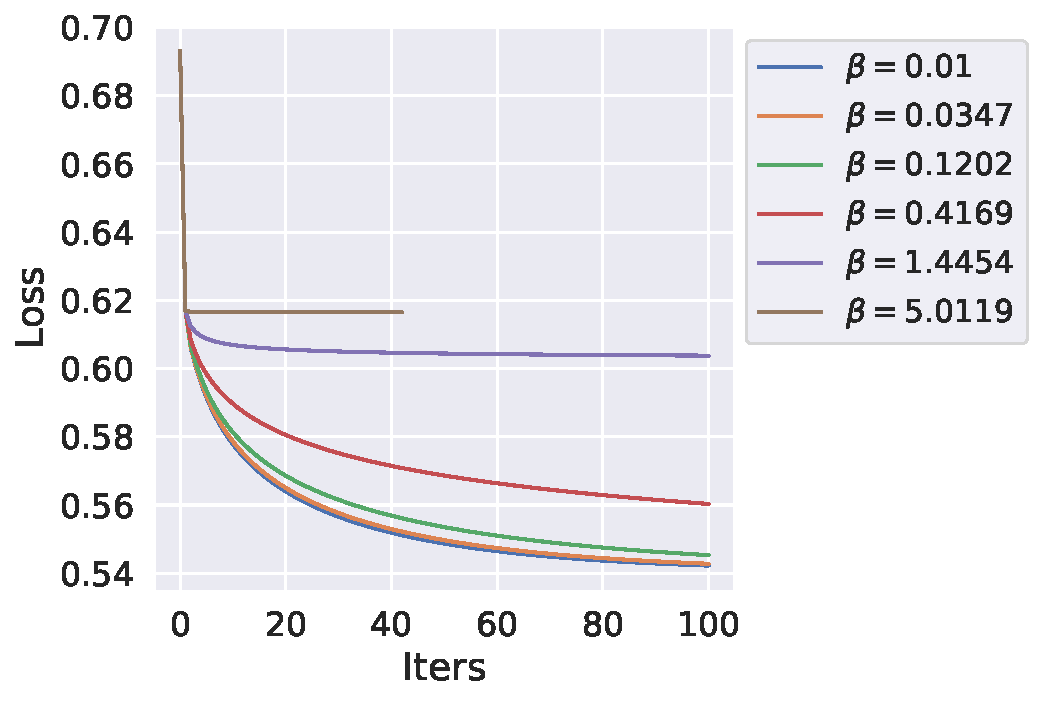
\includegraphics[width=0.5\linewidth]{./experiment1/beta/gd_loss__iters.pdf}
		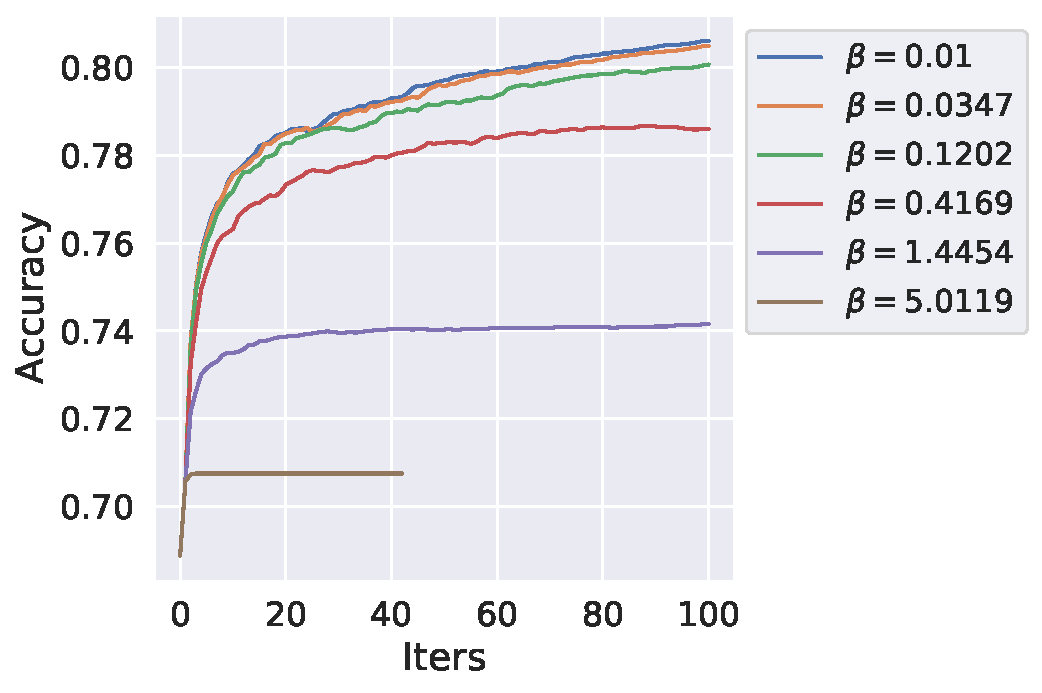
\includegraphics[width=0.5\linewidth]{./experiment1/beta/gd_acc_iters.pdf}
		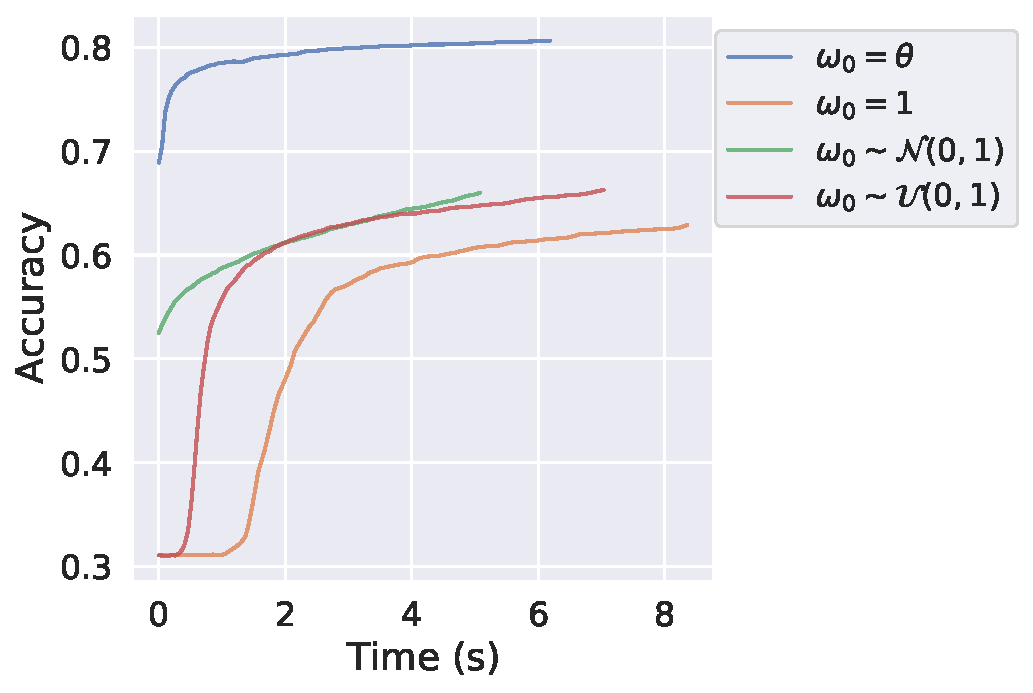
\includegraphics[width=0.5\linewidth]{./experiment1/w_0/gd_acc_time.pdf}
	}
\end{figure}

\begin{figure}[h]
	\centering{
		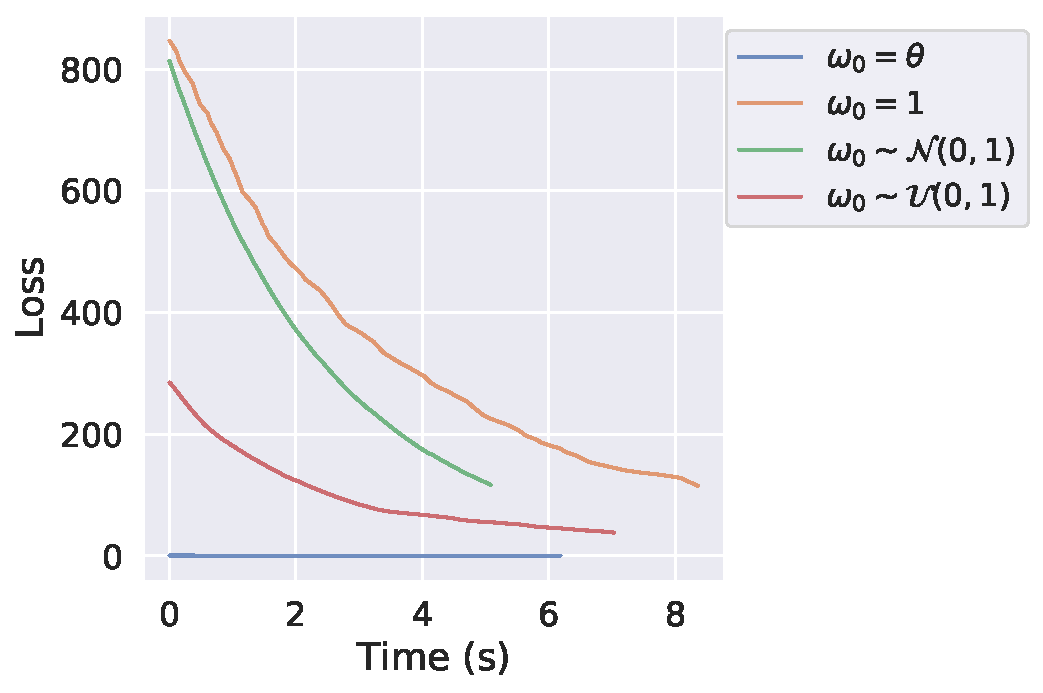
\includegraphics[width=0.5\linewidth]{./experiment1/w_0/gd_loss_time.pdf}
	}
\end{figure}
\newpage
\section{Приложение Б. Стохастический градиентный спуск.}
\begin{figure}[h]
	\centering{
		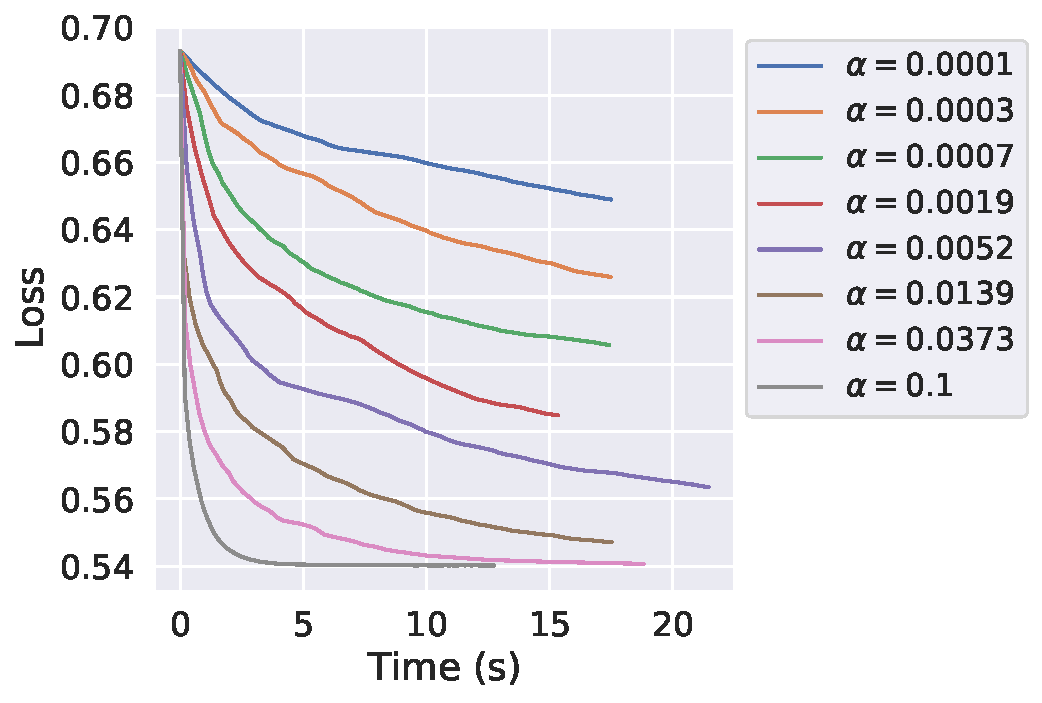
\includegraphics[width=0.5\linewidth]{./experiment2/alpha/sgd_loss_time.pdf}
		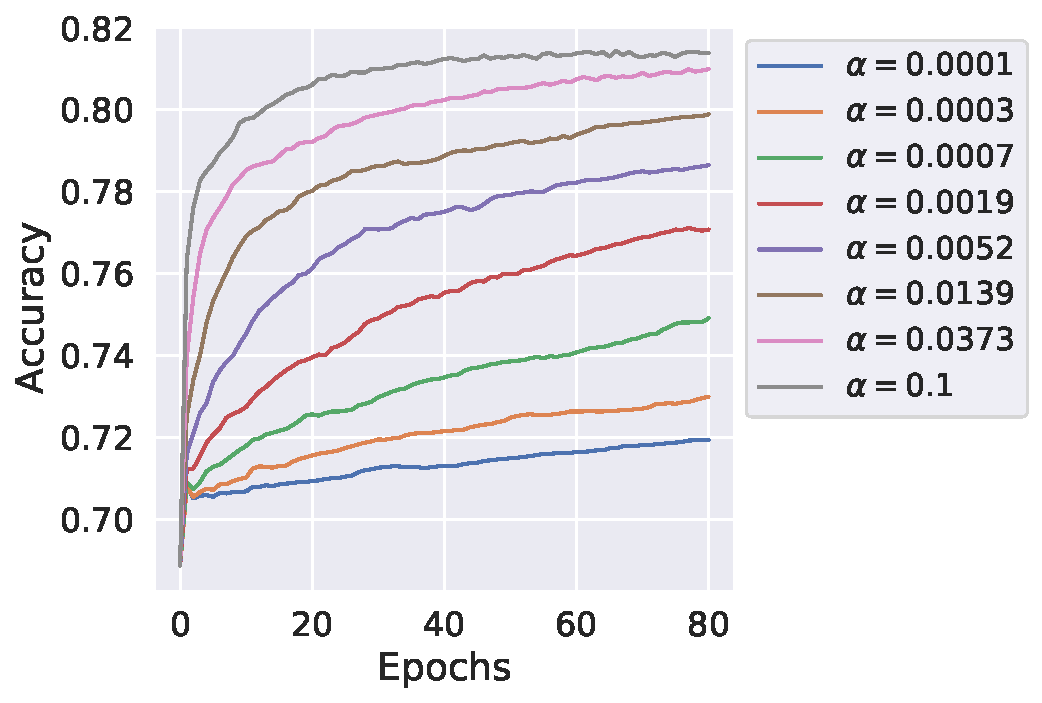
\includegraphics[width=0.5\linewidth]{./experiment2/alpha/sgd_acc_iters.pdf}
	}
\end{figure}
\begin{figure}[h]
	\centering{
		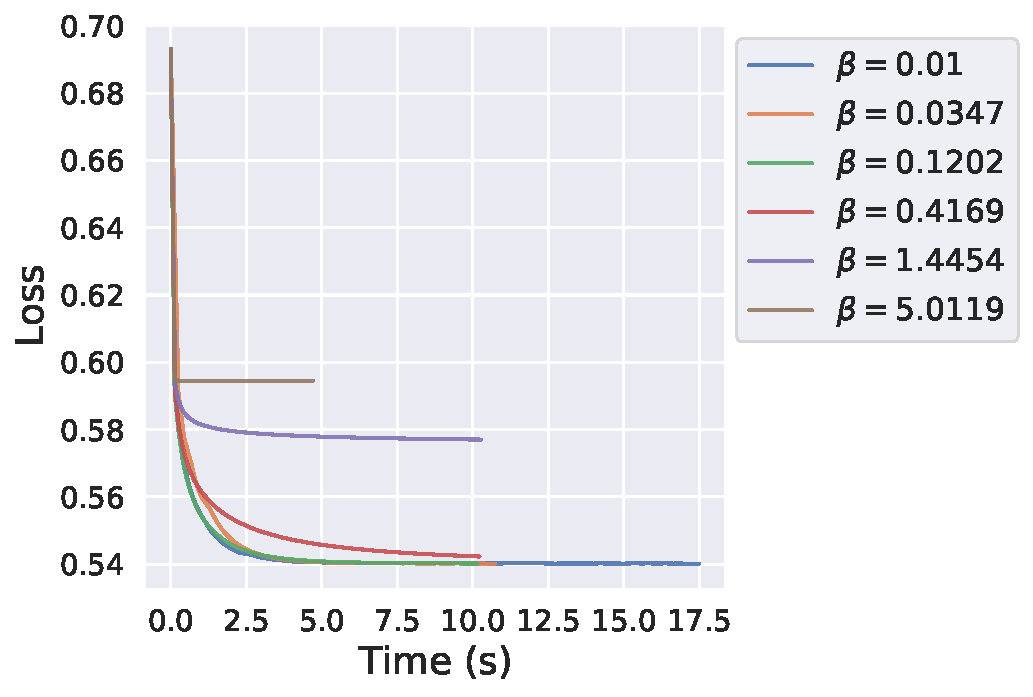
\includegraphics[width=0.5\linewidth]{./experiment2/beta/sgd_loss_time.pdf}
		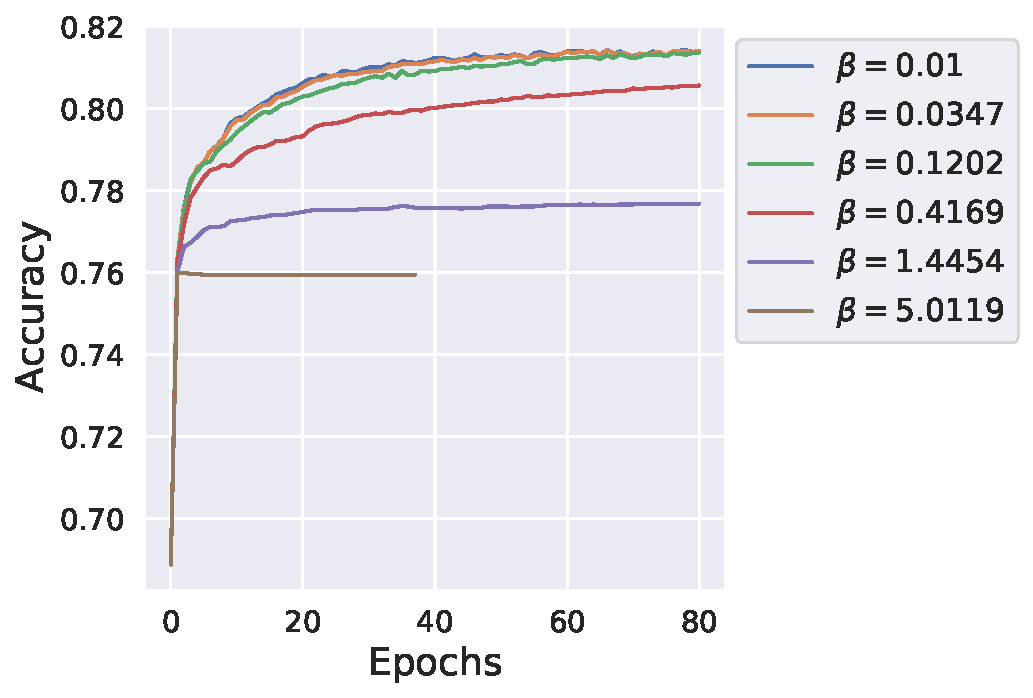
\includegraphics[width=0.5\linewidth]{./experiment2/beta/sgd_acc_iters.pdf}
		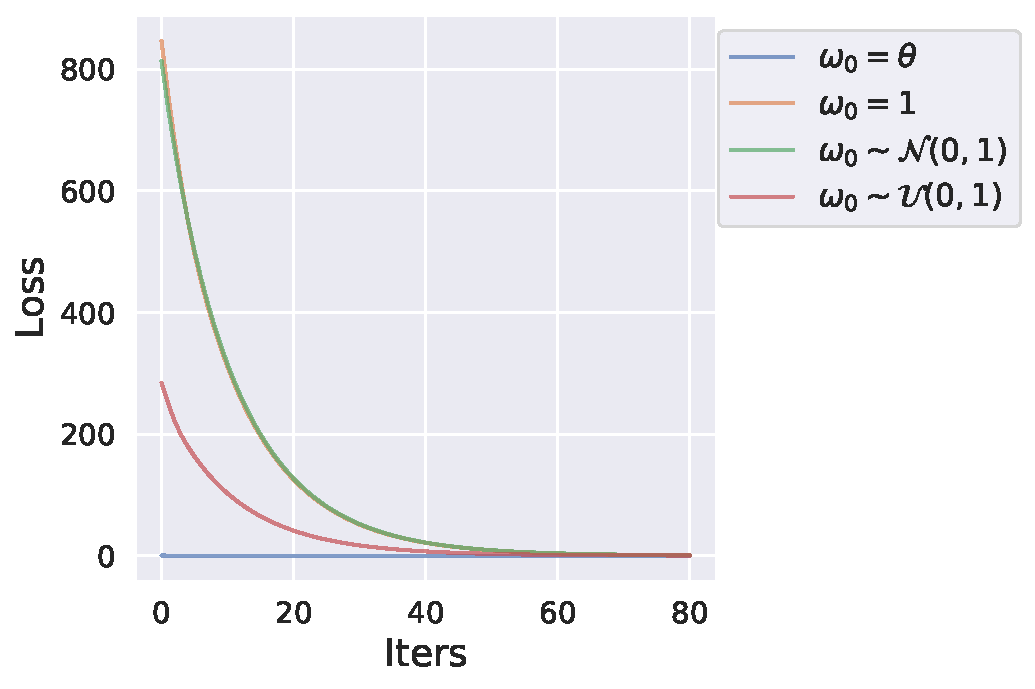
\includegraphics[width=0.5\linewidth]{./experiment2/w_0/sgd_loss_iters.pdf}
		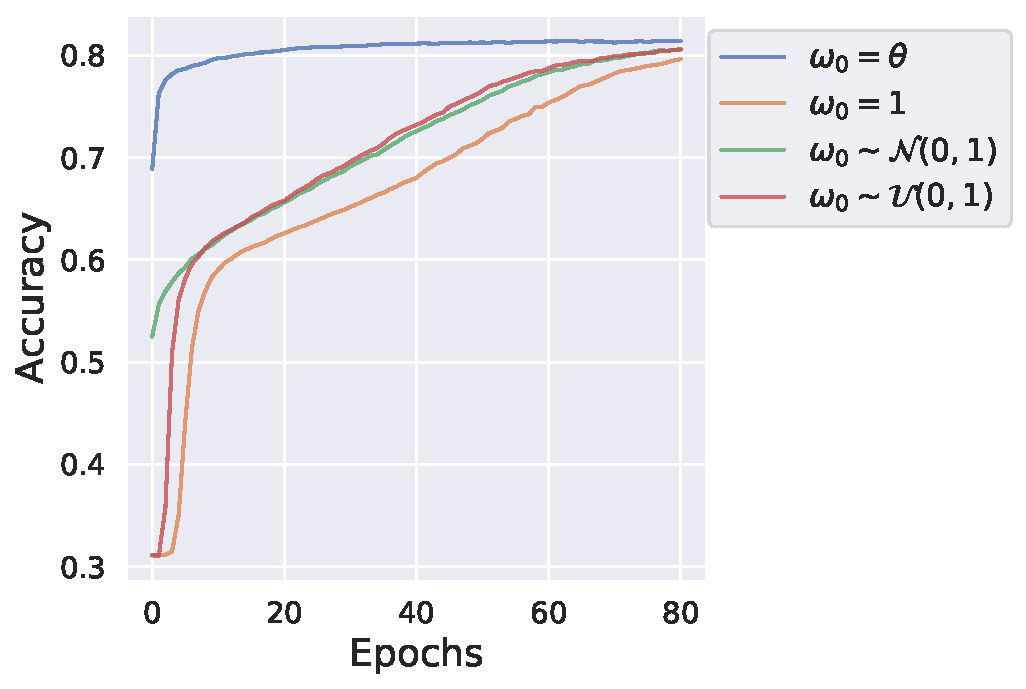
\includegraphics[width=0.5\linewidth]{./experiment2/w_0/sgd_acc_iters.pdf}	
	}
\end{figure}

\begin{figure}[h]
	\centering{
		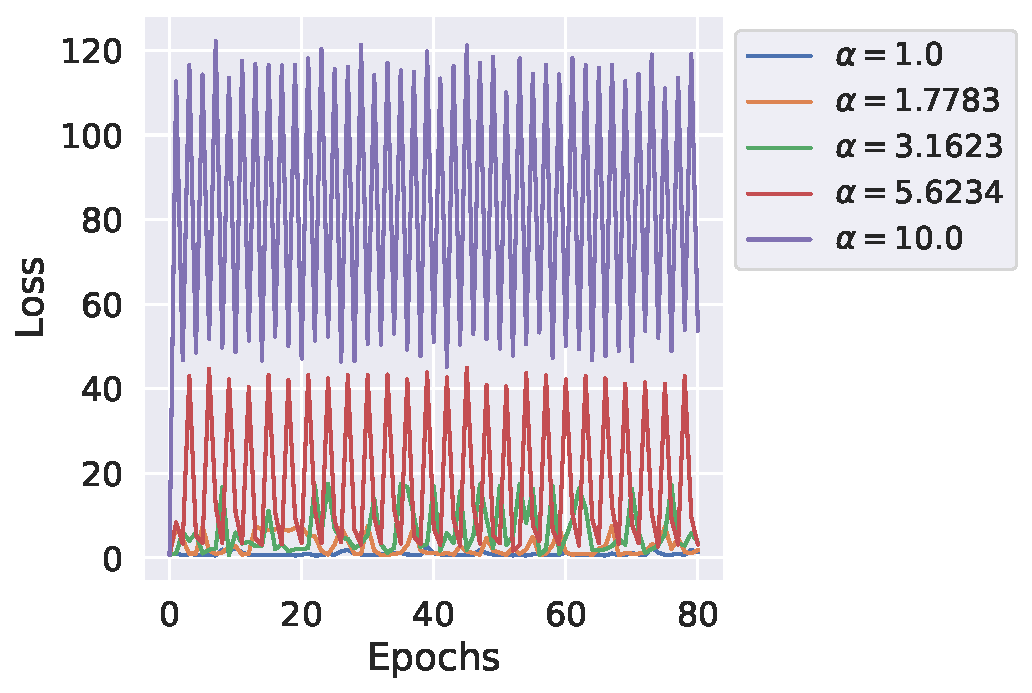
\includegraphics[width=0.5\linewidth]{./experiment2/alpha/sgd_loss__iters_big_alphas.pdf}
		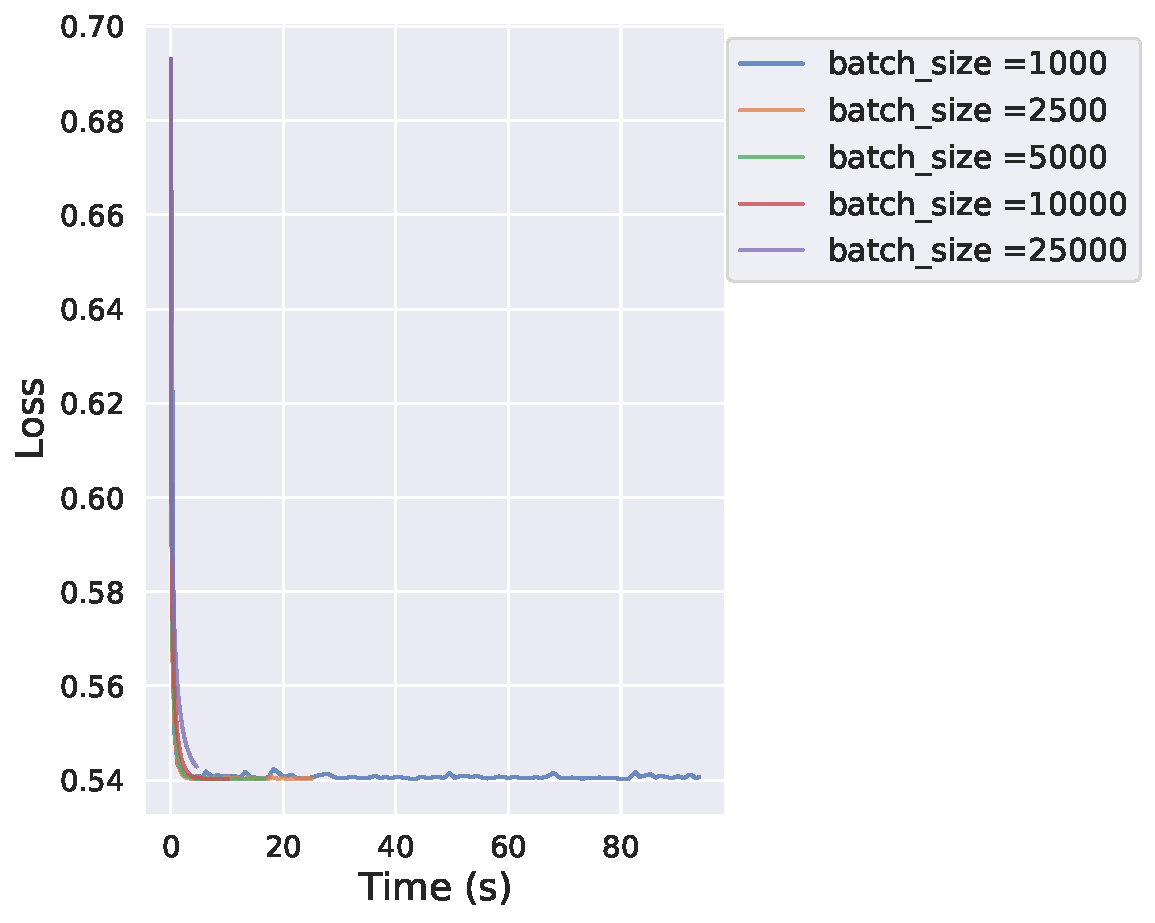
\includegraphics[width=0.5\linewidth]{./experiment2/batch_size/sgd_loss_time.pdf}
		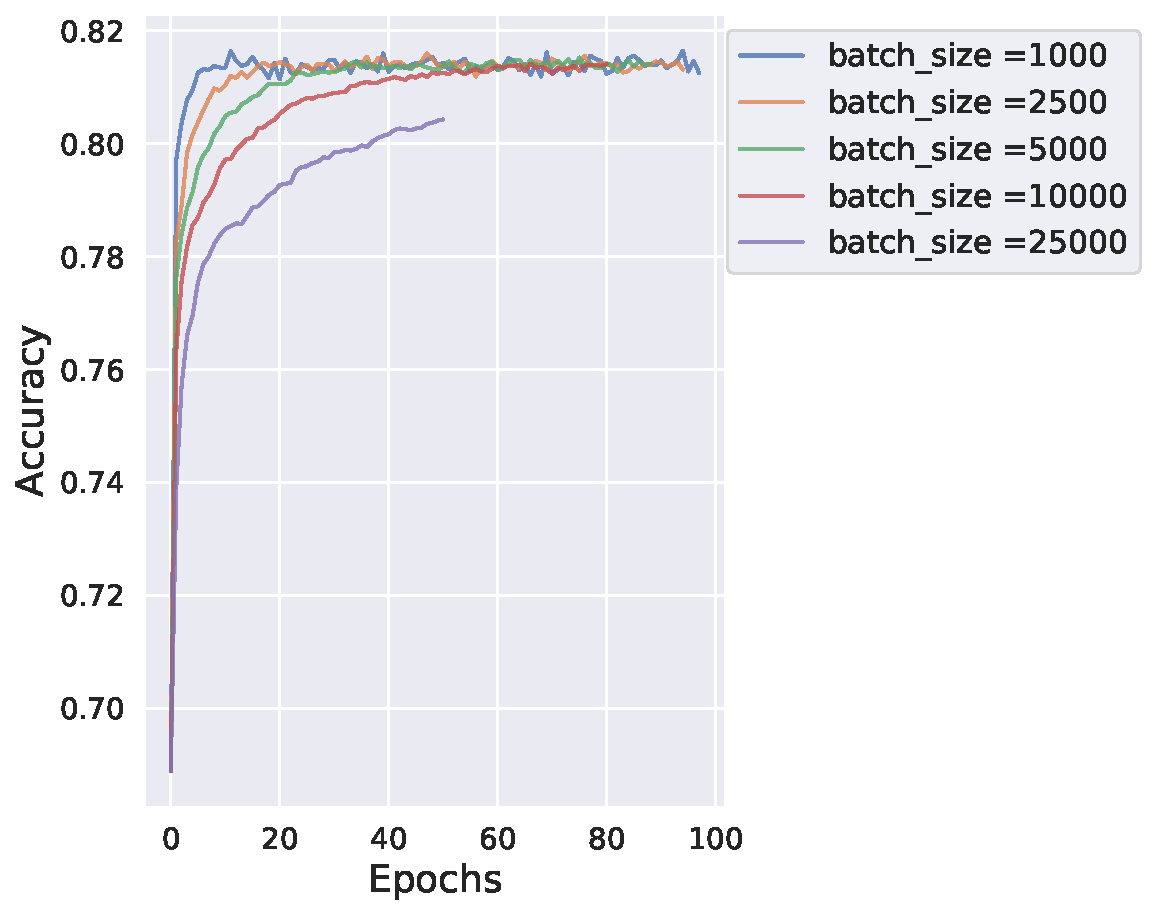
\includegraphics[width=0.5\linewidth]{./experiment2/batch_size/sgd_acc_iters.pdf}
	}
	
\end{figure}
\end{document}